\documentclass[11pt]{report} 
\usepackage{graphicx}
\usepackage{amsmath}
\usepackage{amssymb}
\usepackage[utf8]{inputenc}
\DeclareUnicodeCharacter{03A9}{<LaTeX equivalent>}
\DeclareUnicodeCharacter{039B}{<LaTeX equivalent>}
\usepackage{biblatex}
\addbibresource{references.bib}
\usepackage{float}
\numberwithin{equation}{chapter}

\usepackage{geometry}
\geometry{
  a4paper,
  total={180mm,240mm},
  left=30mm, 
  right=30mm,
  top=25mm,
}
\begin{document}
\begin{titlepage}
   \begin{center}
    
\includegraphics[width=0.8\columnwidth]{Images/nottingham-logo.png} 
    \vspace*{2cm}
    \Huge\\
    
    \textbf{Bigravity Braneworlds}
    
    \vspace{2cm}
    \Large
    A Thesis Submitted in Partial Fulfilment\\
    of the Requirements for the Degree of\\
    Master in Science\\
    
    \vspace{0.7cm}
    by\\
    \vspace{0.5cm}
    \textbf{Matthew Dwyer and Matthew Barnes}
    
    \vspace{0.7cm}
    \large  
    Physics and Astronomy Department\\
    The University Of Nottingham\\
    May 2023
            
   \end{center}
\end{titlepage}
\begin{abstract}
    The cosmological constant and hierarchy problems remain a thorn in General Relativity's side. Physicists have been studying modifications of Einstein's theories for almost as long as they have existed and in this paper we present a particular variation that could potentially solve the aforementioned problems. We will study the Randall-Sundrum 1 model and demonstrate how the warping of the 5-dimensional bulk can eliminate the hierarchy between the fundamental scales. We introduce a bimeric theory of gravity and show that under certain constraints, a theory of non-trivially interacting massive and massless gravitons can be constructed that would negate the need for a dark energy component. We then incorporate the two models addressing both the cosmological constant problem and the hierarchy problem simultaneously. We outline a potential method for deriving viable solutions in the combined theory and discuss the implications and limitations of such a model.
\end{abstract}


\tableofcontents

\newpage

\chapter{Introduction, Motivation, and Summary}

\section{General Relativity}
General relativity or GR, formulated by Albert Einstein in 1915\cite{GR}, fundamentally altered the prevailing understanding of gravity and was a leap of insight that revolutionised physics. It replaced the Newtonian description of gravity with a geometric interpretation, where gravitation arises from the differential geometry of curved spacetime as it is warped by the distribution of mass and energy placed inside it. At the time of its introduction, physicists were grappling with the limitations of classical mechanics and electromagnetism, which had been shown to be inconsistent with one another. Special relativity, the predecessor to the general theory, reconciled these issues with the establishment of the invariance of the speed of light. General relativity extended these principles by incorporating gravity into the framework of spacetime. Einstein's field equations, which are the core of general relativity, are a set of ten partial differential equations that connect the spacetime metric tensor to the stress-energy-momentum tensor. These equations offer a highly non-linear, intricate description of gravitation, in stark contrast to the linear, action-at-a-distance picture provided by Newtonian gravity. The superior nature of general relativity was further demonstrated by its ability to resolve long-standing issues, such as the anomalous precession of Mercury's perihelion, which defied explanation within the Newtonian framework. Additionally, general relativity predicted novel phenomena, such as gravitational time dilation, frame-dragging, and the existence of event horizons in black holes. These predictions have since been confirmed through various experimental and observational evidence, solidifying general relativity as the prevailing theory of gravity\cite{GRTests}. Despite the obvious successes of General Relativity, there exist problems that the theory fails to answer, suggesting that general relativity requires modification.

\section{Two Key Challenges in Gravitational Physics}
Despite its successes, general relativity is not perfect and encounters problems that it fails to address. Two notably persistent issues that continue to challenge researchers are the cosmological constant problem\cite{CCreview} and the hierarchy problem\cite{hierarchyreview}. These failures have become a driving force for modern physicists, motivating them to investigate new modifications to General Relativity. The ultimate goal is to find plausible answers to these perplexing questions, paving the way for a new field in theoretical research referred to as modified gravity. The cosmological constant problem and the hierarchy problem in particular are central to the ideas we explore in this paper, making it essential to gain an understanding of the nature of these two problems and their significance in the field of modified gravity.

\subsection{The Cosmological Constant Problem}
If we study the observations used to estimate the expansion of the Universe, such as Type 1A Supernovae \cite{Perlmutter_1999}, we see the expansion of the universe to be accelerating with a small value of the cosmological constant and is in accordance with a cold Dark Matter scenario where the vacuum energy density is roughly $\Lambda_{obs} = {10}^{-120}M_{PL}$ \cite{Kurts_review}, when measured in Planck units, and presents a contradiction between theory and observation. In Quantum Field Theory, we know that vacuum energy refers to the underlying background fluctuations that exist in empty space, even in the absence of matter or radiation. The concept arises from the principles of Quantum Field Theory of the standard model, which describes particles and their interactions through the framework of fields that permeate all of spacetime. These fields exhibit fluctuations even in their lowest energy state, known as the vacuum state. As a consequence, the fields exhibit a non-zero, minimal amount of energy called zero-point energy that we can calculate, sum together and find the expected vacuum energy density. Herein lies the problem\cite{CCreview}. The implication of General Relativity, mass-energy equivalence, suggests that if there is a vacuum energy then it should warp spacetime, produce a gravitational force, and contribute to the cosmological constant. Performing such a calculation gives us the theoretical expectation value for the cosmological constant to be $\Lambda_{theory}={10}^{-60}M_{PL}$ \cite{RevModPhys.61.1}, a concerning 60 orders of magnitude larger than the observed value. This contradiction has concerned physicists for decades and has been referred to as the largest discrepancy between theory and experiment in all of Physics, and became known as the Cosmological Constant problem. Furthermore, there is no possible dynamical solution to the cosmological constant problem that exists within General Relativity and is evidence that we need to modify it if we wish to find such a solution. Many theories of modified gravity look to produce self-accelerating solutions, which would explain the acceleration of the expansion of the universe without the need for a dark energy component.

\subsection{The Hierarchy Problem}

The Hierarchy problem is the name physicists give to several problems concerning the energy scales of the fundamental forces, and the hierarchy between them. In particular, we ask why there is such a large difference between the size of the Planck scale, $M_{pl} \approx 10^{18}$GeV, and the weak scale, $M_{ew} \approx 10^3$GeV\cite{hierarchyreview}.

Another description of the hierarchy problem arises when we consider the discrepancy between the observed value of the Higgs mass and the Planck mass. Using the quantum field theory of the standard model, we know the non-zero Higgs field is responsible for providing the Fermions with mass terms. We can calculate the mass of the Higgs particle, where we expect the mass to receive contributions of all energy scales up to the cutoff energy, the Planck scale, beyond which the Standard Model begins to break down \cite{Figures}. Then an obvious choice for the scale of the Higgs mass would be the Planck mass. However, observation shows the Higgs mass to be around $250$GeV\cite{hierarchyreview}, which is of the order of the Weak scale and shows another contradiction between theory and observation. This contradiction and the discrepancy between the Planck Scale and the weak scale is the Hierarchy problem. Physicists are yet to find an explanation for the hierarchy that exists between the fundamental energy scales and this remains a primary motivation for modified theories of gravity. There have been different approaches to solving the problem. One approach, and the approach taken in this paper, is through higher dimensional theories of modified gravity where we can create a scenario in which gravity permeates $D$ dimensions whilst confining all other fundamental forces to a $D-1$ dimensional sub-manifold. We then study the behaviour of gravity in such a framework, hoping to eliminate the hierarchy at a fundamental level whilst obtaining an effective theory that reproduces it and is consistent with observation. Specifically, we will look at the Randall Sundrum model, a braneworld scenario, where a potential solution to the hierarchy problem can be found. 
 
\section{Modifying Einstein}
 These challenges, among others, have prompted physicists to explore modifications to the theory that either eliminate the problems or provide a natural explanation for their existence and, after more than a century from the release of Einstein's original papers, there are now a plethora of proposals of modified theories. One of the relatively simpler examples of such theories is $f(R)$ gravity, which modifies the Einstein-Hilbert Action\cite{fr_review}, 
 \begin{equation}
     S = \frac{1}{2\kappa}\int  R \sqrt{-g}d^4 x
 \end{equation}
 by, unsurprisingly, replacing the linear dependence on the Ricci scalar with a more general function, $f(R)$, as follows
 \begin{equation}
     S = \frac{1}{2\kappa}\int  f(R) \sqrt{-g}d^4 x
 \end{equation}
 As such, $f(R)$ is actually a family of many different theories that make different choices for this function. The implications of this seemingly subtle change are dramatic, as it results in vastly different field equations that are fourth-order in the metric tensor derivatives, in contrast to the second-order equations in General Relativity and suggests early and late-time universe expansion without invoking dark matter or dark energy. $f(r)$ is not experimentally viable however and we can show this from the modified Einstein-Hilbert action (1.2). Rewriting the Ricci-scalar function using a Lagrange multiplier,
 \begin{equation}
     S = \int d^4x \sqrt{-g}\big[f\left(\phi\right)-\lambda\left(R-\phi\right)\big]
 \end{equation}
 If we vary with respect to $\lambda$ we recover (1.2), however varying with respect to $\phi$ yields
 \begin{equation}
     f^{\prime}\left(\phi\right)-\lambda=0
 \end{equation}
 We can substitute this back into (1.3) we are left with,
 \begin{equation}
     S=\int d^4x \sqrt{-g} f^{\prime}\left(\phi\right)R
     +\big[f\left(\phi\right)-f^{\prime}\left(\phi\right)\phi]
 \end{equation}
 Which is just a scalar-tensor theory or Brans-Dicke theory with $w=0$ and is not observationally viable\cite{bransdicke}. This is an example that we should bear in mind as we consider our theory of modified gravity. We must take care when constructing our model to avoid instabilities like ghosts and ensure they fall in line with experimental observations. 
 
\subsection{Higher-Dimensions}
A second famous modification made to gravity was a forerunner in a class of theories that invoke higher dimensions and is known as Kaluza-Klein theory. Its origins date back almost as old as Relativity itself when, in 1919, a German Physicist by the name of Theodor Kaluza was studying Einsteins' equations and realised that if he were to solve them in 5-Dimensions, as opposed to the conventional 4, then Maxwell's equations for Electromagnetism emerge naturally from the analysis \cite{1921SPAW.......966K}. Shocked by this unexpected result, Kaluza wrote to Einstein to share his discovery who encouraged him to publish his findings, which Kaluza later did. Surprisingly, however, Kaluza's work was not picked up by other Physicists of the time and it wasn't until 1926 when Oscar Klein contributed a quantum formulation of the theory for the field to gain more significant interest. In his original theory, Kaluza added a constraint called the cylinder condition that forbids any component of the new 5-dimensional metric from depending on the introduced 5th dimension, which was necessary for two reasons. Firstly, the corresponding field equations become vastly more complex without it and, secondly, normal 4-dimensional gravity seems to exhibit this condition naturally. The constraint was later given the physical interpretation by Klein who suggested it implied the 5th dimension was small, compact, and curled up on the scale of around $10^{-33}cm$ \cite{Klein1926TheAO}. Klein's quantum interpretation also introduced so-called "Kaluza-Klein modes" which are the quantised vibrational modes or excitations of fields (such as the electromagnetic field) that exist in this extra compact dimension, with different modes corresponding to different energy levels. These modes manifest as discrete particles or fields in our familiar four-dimensional spacetime. Kaluza-Klein established itself as a pioneering theory, laying the foundation as a precursor for numerous contemporary scientific investigations.\\

Higher-dimensional theories have remained in vogue in the decades since, but interestingly, one of the most well-known uses of extra dimensions today emerged entirely by chance. During the 1960s, physicists at CERN were working to try and understand the strong interaction\cite{stringreview}. Whilst there was already a theory that worked very well at this point, Quantum Electrodynamics, the issue was that this theory only applied to the interactions between electrons and photons and not the ever-growing class of Hadrons that were being discovered. The 'accident' that these investigations resulted in was String theory and, although having to overcome many pitfalls and challenges along the process, it was fine-tuned into the controversial but promising framework for Unification that it is today. Higher dimensions arose naturally from the development of string theory as a necessity for it to be fully consistent with General Relativity. In fact, modern M-Theory (the overarching structure that encompasses numerous string theories) is an 11-Dimensional theory\cite{Mtheory} that generalises Kaluza-Klein such that the extra dimensions are small and compactified. The study of strings also brought about the implementation of mathematical objects called Branes which have been employed in various incarnations within the field, including the research presented in this paper. Braneworlds, or "branes", are theoretical hypersurfaces of varying dimensions that can be treated as surfaces that are embedded within the higher-dimensional structure of spacetime. A crucial property of branes in String Theory is their ability to satisfy Dirichlet boundary conditions by serving as the boundaries of open strings where the strings' endpoints are on the branes \cite{Polchinski_1995}. This aspect is particularly significant when attempting to explain how fundamental forces such as electromagnetism, and weak and strong nuclear forces are restricted to our four-dimensional spacetime, while gravity can operate across all dimensions. In the context of M-Theory\cite{Mtheory}, the "Braneworld" scenario is considered, where our four dimensions are envisioned as existing on a brane embedded within a larger 11-dimensional manifold, known as the Bulk. The dynamics of branes are governed by a set of equations derived from the principle of least action, which considers the tension or energy of the brane and any external fields acting on it. Branes are an essential concept in modern theoretical physics, providing a versatile framework for investigating the structure and interactions of particles and forces in a higher-dimensional spacetime.

\subsection{Randall-Sundrum}
The Braneworld scenario is central to the ideas in this paper. In particular, we consider the Randall-Sundrum Braneworld models, Randall-Sundrum 1 (RS1) and Randall-Sundrum 2 (RS2), released in two forms over two papers in 1999 titled "A Large Mass Hierarchy from a Small Extra Dimension"\cite{RS2} and "An Alternative to Compactification"\cite{RS1}. Each paper proposed a similar but distinct Braneworld model that envisions our Universe as existing on a (3+1)-dimensional Brane that is embedded within a 5-dimensional Bulk that is warped drastically. The model of the first paper, RS1, comprises two branes, at fixed points in the manifold, separated by a finite slice of $AdS_5$ space, with the branes forming the domain walls to this space and the bulk exhibiting $\mathbb{Z}_2$-symmetry centered on each of the branes.

\begin{figure}[h]
\centering
    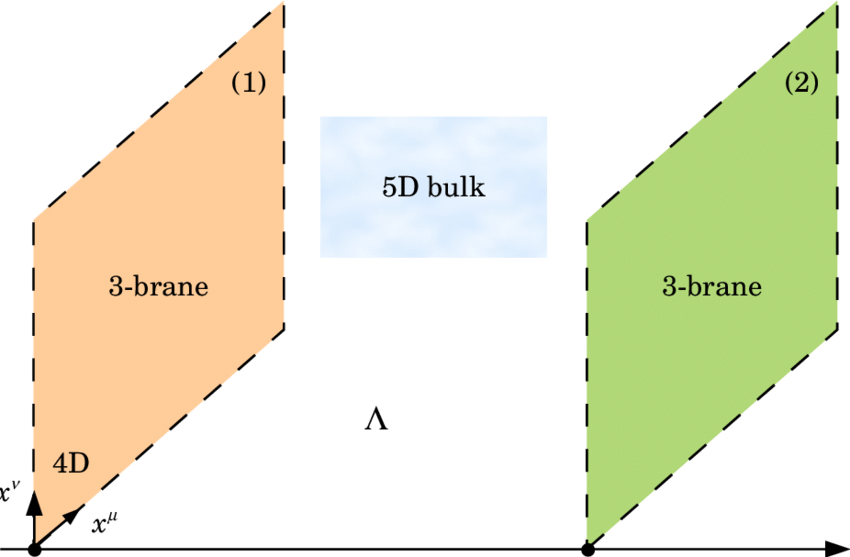
\includegraphics[scale=0.25]{Images/RS1.png}
    \caption{The RS1 Model\cite{RS1Diagram}.}
    \label{fig:RS1}
\end{figure}
One brane is called called the Planck Brane, where gravity is much stronger, and the other is called the Tevbrane, where gravity is much weaker and also where our universe and the Standard model fields are localised. Gravity is much weaker on the Tevbrane due to the presence of a warp factor introduced into the metric for the model. Gravity is not confined to the branes but is instead allowed to freely propagate into the extra dimension and the large warping of the Bulk in this model presents a solution to the hierarchy problem.

The second model, RS2, differs from RS1 because brane separation is extended to infinity. The Tevbrane is effectively removed from the physical model and so we are left with a single brane, the Planck Brane, with the bulk exhibiting the same  $\mathbb{Z}_2$-symmetry centered about it. In this model, our universe exists on the remaining brane with the important distinction that the graviton's probability function does not fall as we move away from the Planck brane as it does in RS1 but is instead bound to the single brane. 
The RS2 model is interesting as it demonstrates how Newton's 4-Dimensional gravity can be recovered in a 5-Dimensional model without the need for the extra dimension to be small. This is of particular interest for the AdS/CFT conjecture, though it will not be explored in this paper.\\

The Randall-Sundrum Braneworld scenarios are set apart from other higher-dimensional theories as they involve a unique solution to Einstein's equations. Specifically, a non-factorisable metric of the form
\begin{equation}
ds^2= dz^{2} + a^{2}(z) q _{\mu\nu}(x) dx^{\mu} dx^{\nu}   
\end{equation}
where the metric for $x^{\mu}$ and $x^{\nu}$ is not independent of the coordinates of the 5th additional dimension of the bulk, $z$, which was prohibited in other theories like Kaluza-Klein with the introduction of the cylinder condition. The dropping of this assumption is essential for the natural hierarchy mentioned previously, as we shall see later on in our analysis of the RS1 model. \\

\begin{figure}[h]
\centering
    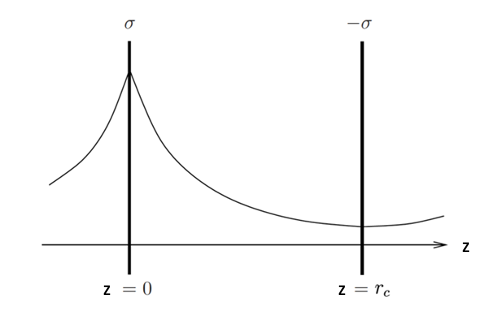
\includegraphics[scale=0.6]{Images/RS1 warp factor.png}
    \caption{A Plot of the Warp Factor in the RS1 Model, where $r_c$ is the distance form the brane centered at $y=0$ \cite{Figures}.}
    \label{fig:RS1}
\end{figure}

\subsection{Massive and Bimetric Gravity}
Introduced by Wolfgang Pauli and Markus Fierz in the first half of the 20th century \cite{fierz1939relativistic}, massive gravity is a deformation away from classical GR by providing the graviton with a mass term. \\
As a modified theory of gravity, massive gravity looks to solve the problems that general relativity is faced with. Many theories of modified gravity often face criticism when attempting to solve the cosmological constant problem since most proposed solutions don't explain where the small value of the cosmological constant has come from. Solutions are often unnatural and rather just shift the fine-tuning of the constants into other parameters \cite{Kurts_review}. Massive gravity might have a natural solution to the cosmological constant problem. If a parameter is technically natural, it will have a symmetry that appears as the parameter tends towards zero and protects it against quantum corrections. Massive gravity introduces a mass term to the graviton which breaks the gauge symmetry of GR which we know to be general coordinate invariance. As we set the graviton mass back towards zero we recover general coordinate invariance, introducing a gauge symmetry that protects against quantum corrections and allows us to find a technically natural solution to the cosmological constant problem. This unique feature makes massive gravity an attractive area of research in the ongoing quest to better understand the fundamental nature of gravity and its role in shaping the universe. \\

Since Fierz and Pauli, massive gravity has become a field of research with many different variations and approaches, introduced to solve the issues that earlier theories encountered. Discontinuities and instabilities plagued Fierz-Pauli and other early theories, requiring new liberating theories like the de Rham-Gabadadze-Tolley (dRGT) theory of massive gravity \cite{de_Rham_2010} \cite{de_Rham_2011}. 

\noindent In this project, we are interested in looking at the "Bimetric" extension of Massive gravity in particular. Bimetric gravity is a class of modified gravitational theories that incorporates two interacting metrics in the Einstein-Hilbert action and its history traces back to the early 20th century, following the success of General Relativity when Physicist Nathan Rosen\cite{PhysRev.57.147}\cite{PhysRev.57.150}, a collaborator of Einstein, proposed a model of spacetime where for every point there were two associated metrics. The idea of extending the single metric of General Relativity to add an additional "fiducial" metric has attracted attention from several researchers over the years, with various iterations of models being proposed \cite{PhysRevD.80.123536}. The primary motivation behind these models has been to address unresolved questions in cosmology and astrophysics, such as the nature of dark energy, dark matter, and the Cosmological Constant problem mentioned previously. Bi-metric theories experienced renewed interest in the late 20th and early 21st centuries due to de Rham, Gabadadz and Tolley's new formulation and remains one of the forerunning theories in Massive Gravity. 

\section{An Outline of our Work}
This paper focuses on finding a viable phenomenology of a bimetric theory of gravity in the Randall - Sundrum 1 braneworld scenario. We begin by introducing the Randall-Sundrum braneworld models in Chapter 2, focusing heavily on the RS1 model. In this chapter, we set up the RS1 model before looking at the dynamics of spacetime in the bulk and discuss a solution to the hierarchy problem and end the chapter with a brief discussion of the RS2 model. In Chapter 3, we introduce theories of massive gravity and aim to provide some motivation for their study. We will discuss some of the prerequisites to bimetric gravity and end the chapter by exploring bimetric theory in depth. Chapter 4 will aim to incorporate bimetric gravity into our RS1 braneworld scenario. We decouple one metric from matter and first look to find solutions when there are no interactions between the two metrics. We then introduce the interaction terms by perturbing the non-interacting case and aim to derive background solutions. Currently, no solutions have been found in the interacting case, if solutions are found this constitutes novel research. In Chapter 5 we will present a summary of our findings along with an analysis of its successes and potential pitfalls. We will discuss potential routes for experimental verification and suggest avenues for future research.

\chapter{Randall-Sundrum Braneworlds}
The Randall-Sundrum (RS) braneworld models have gained significant attention in theoretical research due to their innovative approach to solving the hierarchy problem and presenting an alternative to conventional compactification schemes. Moreover, RS braneworlds hold crucial conceptual significance in braneworld-related studies and are frequently encountered in advanced areas of physics, including holography, conformal field theory, supersymmetry, and other frontiers of the field. As a result, RS braneworlds have become a focal point in modern physics. This chapter will establish the foundations of RS braneworld models whilst highlighting their unique attributes. We study a generalisation of RS1, where we allow the branes to have intrinsic curvature, and present the dynamics of the bulk. We then present a solution to the hierarchy problem and end the chapter with a discussion of the RS2 model. 
\section{RS1}
To begin, let us first set up the framework for our Randall-Sundrum 1 (RS1) model. The RS1 model introduces an extra dimension, $z$, to our 4d universe. The extra dimension is compactified on an $S^1/\mathbb{Z}^2$ orbifold, so that it has circular $S^1$ topology with fixed radius and a 'mirror' $\mathbb{Z}^2$ symmetry about its end points, so that both sides of the circle are in equivalence. We have two key points in the orbifold, $z=z_1$ and $z=z_2$, where a domain wall is fixed at each point. These domain walls are 3-branes, 4d submanifolds with 4d brane coordinates $ {\{ \zeta^\mu\}} $. The extra dimension $z$ points tangential to the branes and therefore the  ${\{ \zeta^\mu\}}$ coordinates. Each brane will have an associated metric, $\gamma_1$ and $\gamma_2$, where the index identifies the brane.

We will label the brane at $z_1$ as the Planck brane and the brane at $z_2$ the TeV brane. We imagine that we are observers inside the TeV brane, which comprises the 4d universe we experience and exist in. All standard model fields are bound to the TeV brane, but gravity can freely propagate into the extra dimension. The 5d space between the Planck brane and the TeV brane is known as the bulk.

This model will consider configurations of the form,
\begin{equation}
    ds^2= N^2(z)dz^{2} + a^{2}(z) q _{\mu\nu}(x) dx^{\mu} dx^{\nu}
\end{equation}
where we have a 4d non factorisable, maximally symmetric metric $q_{\mu\nu}dx^\mu dx^\nu$ with extrinsic curvature $\lambda$, scaled by a 'warp factor' $a(z)$, which is a function of our extra dimension. The extra dimension is scaled by a lapse function $N(z)$, which controls the size of the extra dimension. We identify our coordinate system $X^a = (x^\mu , z)$ and our brane coordinates $\zeta^\mu = x^\mu$ e.g at $z=z_1$, the brane metric $\gamma^{1}_{\mu\nu}=a^{2}(z_1) q _{\mu\nu}(x)$. Note that we use the notation convention that Greek indices denote four-dimensional coordinates and Latin indices denote five-dimensional coordinates.\\
From (2.1) we obtain the metric tensor
\begin{equation}
    g_{a b}=a^2(z) q_{\mu\nu}+\delta_a^z \delta_b^z N^2(z)
\end{equation}
The action for the model is as follows \cite{RS1},
\begin{equation}
    S= \int d^{5}x  \sqrt{-g} \bigg\{ \frac{M^{3}_{5}}{2} R -2\Lambda \bigg\}  +S_{branes}
\end{equation}
The first part is an Einstein - Hilbert term, describing the dynamics of an empty Bulk with the addition of a 5d cosmological constant term, $\Lambda$, where $g=det(g_{ab})$ is the determinant of our metric (2.1), $M^{3}_{5}$ is the 5-dimensional Planck mass and $R$ is a 5d Ricci scalar. The final term, $S_{branes}$, is the action for our branes and is defined as
\begin{equation}
    S= -\sigma_1\int d^{4}\zeta   \sqrt{-\gamma_1} - \sigma_2\int d^{4}\zeta   \sqrt{-\gamma_2}
\end{equation}
Where the branes each have a constant energy density known as the brane tensions, $\sigma_1$ and $\sigma_2$, and $\sqrt{-\gamma_1}$ and $\sqrt{-\gamma_2}$ are the determinants of the metrics on those branes.\\

Using this assignment, and the properties of the determinant, our action becomes
\begin{equation}
    S= \int d^{5}x Na^{4} \sqrt{-q} \bigg\{ \frac{M^{3}_{5}}{2} R -2\Lambda \bigg\} - \sigma_1\int d^4x\sqrt{-q}a^4(z_1)\delta(z-z_1) - \sigma_2\int d^4x\sqrt{-q}a^4(z_2)\delta(z-z_2)
\end{equation}
where $a^4(z_1) = a^4(z_2)$ to satisfy continuity conditions on the brane, and we can relabel both terms simply as $a^4(z)$ since the terms will only appear when we are on the branes due to the presence of the accompanying delta functions. Applying this relabelling, the action is
\begin{equation}
    S= \int d^{5}x Na^{4} \sqrt{-q} \bigg\{ \frac{M^{3}_{5}}{2} R -2\Lambda \bigg\} - \sigma_1\int d^4x\sqrt{-q}a^4\delta(z-z_1) - \sigma_2\int d^4x\sqrt{-q}a^4\delta(z-z_2)
\end{equation}
Throughout this paper, it is worth noting that we may suppress $a(z)$ and $N(z)$ simply to $a$ and $N$. This is to simplify notation and in no way changes the structure of either the warp or lapse function.
\subsection{The Ricci Scalar}
To analyse our action we need to find the Ricci Scalar, $R$. First, we need to find the Christoffel connections which will allow us to derive the Ricci tensor and eventually the Ricci scalar. We will employ our usual syntax, where Greek indices represent four-dimensional components and Latin indices represent five-dimensional components. See the appendix for full details of the calculation. Using (2.1), we find the useful properties
\begin{equation}
    \begin{aligned}
& \Rightarrow g_{a b}=g_{a b}(z) \\
& \Rightarrow \partial_\mu g_{a b}=0, g^{z \mu}=0, g_{z \mu}=0
\end{aligned}
\end{equation}
Then we can identify all non-zero Christoffel connections
\begin{equation}
    \Gamma_{\alpha \beta}^\mu= \frac{1}{2} q^{\mu \gamma}(\partial_\beta q_{\alpha \gamma}+\partial_\gamma q_{\beta \alpha}+\partial_\alpha q_{\gamma \beta})
\end{equation}
\begin{equation}
    \Gamma_{\mu \nu}^z= -\frac{a^\prime a}{N^2}q_{\mu \nu} = -\frac{a^\prime}{aN^2}g_{\mu \nu}
\end{equation}
\begin{equation}
    \Gamma_{z \nu}^{\mu} = \Gamma_{\nu z}^{\mu} = \frac{a^\prime}{a}\delta_{\nu}^{\mu}
\end{equation}
\begin{equation}
    \Gamma_{zz}^z = \frac{N^\prime}{N}
\end{equation} 
All other Christoffel connections are vanishing. We have all the necessary ingredients to construct the Ricci tensor, $R_{ac}$, found by contracting the Riemann tensor, $R_{abc}^b$.
\begin{equation}
    R_{ac} = -\partial_{a}\Gamma_{bc}^b + \partial_{b}\Gamma_{ac}^b + \Gamma_{ca}^e\Gamma_{be}^b - \Gamma_{cb}^e\Gamma_{ae}^b
\end{equation}
By inspection, $R_{\mu z} = R_{z\mu}$ vanishes. Then, to calculate the full Ricci tensor we only need $R_{\mu \nu}$ and $R_{zz}$. Using (2.8), (2.9), (2.10), (2.11) and (2.12), we find
\begin{equation}
    R_{zz} = 4\frac{N^\prime}{N}\frac{a^\prime}{a} - 4\frac{a^{\prime\prime}}{a}
\end{equation}
\begin{equation}
    R_{\mu\nu} = q_{\mu\nu}\left(3\lambda - \frac{a^{\prime\prime}a}{N^2} - 3\left(\frac{a^\prime}{N}\right)^2 + \frac{a^\prime aN^\prime}{N^3}\right)
\end{equation}
By contracting the Ricci tensor with the inverse metric, $g^{ab}$, we can calculate the Ricci scalar
\begin{equation}
    R = g^{ab}R_{ab} = g^{\mu\nu}R_{\mu\nu} + g^{zz}R_{zz}
\end{equation}
which yields
\begin{equation}
    R = \frac{12\lambda}{a^2} - 12\left(\frac{a^\prime}{a}\right)^2\frac{1}{N^2}+8\frac{N^\prime}{N^3}\frac{a^\prime}{a}-8\frac{a^{\prime\prime}}{a}\frac{1}{N^2}
\end{equation}
We now substitute the explicit form of the Ricci scalar into (2.6) to obtain a complete action of our model.

\begin{equation}
   \begin{aligned}    
    S = \int dzd^4x\sqrt{-g}\left[-2\Lambda + \frac{M_{5}^3}{2}\left(\frac{12\lambda}{a^2} - 12\left(\frac{a^\prime}{a}\right)^2\frac{1}{N^2}+8\frac{N^\prime}{N^3}\frac{a^\prime}{a}-8\frac{a^{\prime\prime}}{a}\frac{1}{N^2}\right)\right]\\ - \sigma_1\int d^4x\sqrt{-q}a^4(z)\delta(z-z_1) - \sigma_2\int d^4x\sqrt{-q}a^4(z)\delta(z-z_2)
   \end{aligned}
\end{equation}
\subsection{EOMs for $a(z)$ and $N(z)$}
Now that we have the explicit action for our model we can proceed with deriving our equations of motion for the Warp factor and lapse function. This analysis will give us insight into the geometry of the Bulk and will lead us towards a relationship between the tension of the branes and the cosmological constant and further still a solution to the Hierarchy problem. Recalling our action in (2.17)
\begin{multline}
    S=\int\ dzd^4xNa^4\sqrt {-q}\bigg(-2\Lambda+\frac{M^3_5}{2}\bigg(\frac{12\lambda}{a^2}-12\bigg(\frac{a^\prime}{a}\bigg)^2\frac{1}{N^2}+\frac{8N^\prime}{N^3}\bigg(\frac{a^\prime}{a}\bigg)\\ -\frac{8}{N^2}\bigg(\frac{a^{\prime\prime}}{a}\bigg)\bigg)\bigg)-\sqrt{-q}\sigma_1a^4(z)\delta\big(z-z_1\big)-\sigma_2a^4(z)\delta\big(z-z_2\big)
\end{multline}
we can identify the Lagrangian
\begin{multline}
    \mathcal{L}=Na^4\sqrt {-q}\bigg(-2\Lambda+\frac{M^3_5}{2}\bigg(\frac{12\lambda}{a^2}-12\bigg(\frac{a^\prime}{a}\bigg)^2\frac{1}{N^2}+\frac{8N^\prime}{N^3}\bigg(\frac{a^\prime}{a}\bigg)\\-\frac{8}{N^2}\bigg(\frac{a^{\prime\prime}}{a}\bigg)\bigg)\bigg)-\sqrt{-q}\sigma_1a^4(z)\delta\big(z-z_1\big)-\sigma_2a^4(z)\delta\big(z-z_2\big)
\end{multline}
which allows us to use the Euler-Lagrange equation for dependence on second-order derivatives (See Appendix A for details on the derivation),
\begin{equation}
    \frac{\partial\mathcal{L}}{\partial Y}-\frac{d}{dt}\bigg(\frac{\partial\mathcal{L}}{\partial \Dot{Y}}\bigg)+\frac{d^2}{dt^2}\bigg(\frac{\partial\mathcal{L}}{\partial \Ddot{Y}}\bigg)=0
\end{equation}
 This analysis yields the equation of motion for $a(z)$ (see appendix B for details on the derivation)

\begin{align}
    -2N\Lambda+3M_5^3\bigg\{\frac{\lambda}{a^2}-\bigg(\frac{a^\prime}{a}\bigg)^2\frac{1}{N}+&\frac{N^\prime}{N^3}\bigg(\frac{a^\prime}{a}\bigg)-\frac{1}{N^2}\left(\frac{a^{\prime\prime}}{a}\right)\bigg\}=\\ \nonumber
    &-\sigma_1a^3(z)\delta\big(z-z_1\big)+\sigma_2a^3(z)\delta\big(z-z_2\big)
\end{align}
We can simplify this further via a re-scaling of our $z$ coordinates. Looking back at the configuration of our metric, (2.3), we consider the transformation
\begin{equation}
    z\xrightarrow{}f(z)
\end{equation}
which is just a coordinate transformation. Applying this transformation to our metric EQUATION, we get
\begin{align}
ds^2&=N^{2}(f(z)){f^\prime}^2 dz^{2} + a^{2}(f(z)) q _{\mu\nu}(x) dx^{\mu} dx^{\nu}\\   
&=\Tilde{N}^{2}(z)dz^{2} + \Tilde{a}^{2}(z) q _{\mu\nu}(x) dx^{\mu} dx^{\nu} 
\end{align}
where we see that the form of $a(z)$ term is unchanged and is guage invariant. The $N(z)$ term, however, is not gauge invariant and so we can choose f(z) such that $\Tilde{N}(z)=1$. This further implies that $\Dot{\tilde{N}}(z)=0$ and so our equation of motion reduces to 
\begin{multline}
    -2\Lambda+3M_5^3\bigg\{\frac{\lambda}{a^2}-\bigg(\frac{a^\prime}{a}\bigg)^2-\left(\frac{a^{\prime\prime}}{a}\right)\bigg\}=\sigma_1(z)\delta\big(z-z_1\big)+\sigma_2(z)\delta\big(z-z_2\big)
\end{multline}
This is a second-order differential equation for $a(z)$ and is our final form.\\

\noindent We now look to find our equation of motion for $N(z)$ via the same process and we will see that a second equation can also be derived for $a(z)$ from this. We begin with the same Lagrangian as before.
\begin{multline}
    \mathcal{L}=Na^4\sqrt {-q}\bigg(-2\Lambda+\frac{M^3_5}{2}\bigg(\frac{12\lambda}{a^2}-12\bigg(\frac{a^\prime}{a}\bigg)^2\frac{1}{N^2}+\frac{8N^\prime}{N^3}\bigg(\frac{a^\prime}{a}\bigg)-\frac{8}{N^2}\bigg(\frac{a^{\prime\prime}}{a}\bigg)\bigg)\bigg)\\
    -\sqrt{-q}\sigma_1a^4(z)\delta\big(z-z_1\big)-\sigma_2a^4(z)\delta\big(z-z_2\big)
\end{multline}
There are no second-order terms for $N(z)$, so we can use the Euler-Lagrange equation for only first-order dependence
\begin{equation}
    \frac{\partial\mathcal{L}}{\partial Y}-\frac{d}{dt}\bigg(\frac{\partial\mathcal{L}}{\partial \Dot{Y}}\bigg)=0
\end{equation}
Which yields the equation of motion for $N(z)$ (see appendix B).
\begin{equation}
    -2\Lambda +\frac{M^3_5}{2}\left(\frac{12\lambda}{a^2}-12\left(\frac{a^\prime}{a}\right)^2\frac{1}{N^2}\right) = 0
\end{equation}
We can use the same trick as before and choose $f(z)$ such that $\Tilde{N}(z)=1$, which implies that $\Dot{N}(z)=0$ and so our equation of motion reduces to
\begin{equation}
    a^4\left(-2\Lambda+\frac{M^3_5}{2}\left(\frac{12\lambda}{a^2}+12\left(\frac{a^\prime}{a}\right)^2+8\frac{a^{\prime\prime}}{a}\right)\right)-8\frac{M^3_5}{2}\left(\left(\frac{3a^2}{a^\prime}\right)^2+\frac{a^3}{a^\prime}\right)=0
\end{equation}
\begin{equation}
    \Rightarrow -\Lambda+3M^3_5\left(\frac{\lambda}{a^2}-\left(\frac{a^\prime}{a}\right)^2\right)=0
\end{equation}
Which is a first-order differential equation in $a(z)$.
\subsection{The Warp Factor}
Now that we have our equations of motion, our next task is to solve them and calculate $a(z)$ in the bulk. We study a generalisation of the RS1 model and allow the branes to exhibit intrinsic curvature. The consequence is that both branes can have curvature, $\lambda = 0$, $\lambda > 0$ or $\lambda <0$, corresponding to a Minkowski, De-Sitter or anti-De Sitter brane respectively. This is not new and the generalisation was done almost immediately after the RS1 model was first published \cite{Karch:2000ct}. Flat branes are called critical branes whilst branes with non-zero curvature are known as non-critical branes. We consider all three cases of curvature and look to find the form of the warp factor in the bulk in each case.

For RS1 to be a solution to the hierarchy problem, we require the fundamental 5d Planck scale to be of similar size to the fundamental weak scale. By scaling our 4d non-factorisable metric by the warp factor, we also change the fundamental Planck scale when measured as an effective scale on the brane. Following this, we realise the warp factor must decrease as it moves through the bulk in order to produce a smaller effective Planck scale on the TeV brane, which will be of use when we choose an ansatz to solve our equations of motion in the different cases for $\lambda$.
\\
For critical branes, $\lambda = 0$, and (2.25) reduces to 
 \begin{equation}
    -2\Lambda-3M^3_5\left(\frac{a^{\prime\prime}}{a}+\left(\frac{a^\prime}{a}\right)^2\right)=\sigma_1\delta\left(z-z_1\right)+\sigma_2\delta\left(z-z_2\right)
\end{equation}
We are concerned with the behaviour of the warp factor in the Bulk, away from the branes, where the delta functions cause the brane contributions on the right hand side of (2.31) to vanish. It then reduces to
\begin{equation}
    -2\Lambda-3M^3_5\left(\frac{a^{\prime\prime}}{a}+\left(\frac{a^\prime}{a}\right)^2\right)=0
\end{equation}
Using $\lambda = 0$, we can simplify (2.30) to yield
\begin{equation}
    -2\Lambda+6M^3_5\left(-\left(\frac{a^\prime}{a}\right)^2\right)=0
\end{equation}
Since (2.33) is a first-order differential equation, we choose this equation first to solve for $a(z)$ since we only require one constant of integration and will be easier to solve. 

Making note of its form, we choose to substitute an ansatz of $a(z)=Ae^{\pm\kappa z}$ into (2.33), which generates the solution
\begin{equation}
    a(z)=Ae^{\pm\sqrt{\frac{-\Lambda}{3M^3_5}}z}
\end{equation}
where $A$ is a constant of integration and we identify
\begin{equation}
    \kappa = \sqrt{\frac{-\Lambda}{3M^3_5}}
\end{equation}
Note that both solutions are valid 
\begin{equation}
    a_+(z)=Ae^{\sqrt{\frac{-\Lambda}{3M^3_5}}z}
\end{equation}
\begin{equation}
    a_-(z)=Ae^{-\sqrt{\frac{-\Lambda}{3M^3_5}}z}
\end{equation}
and are in correspondence with the $\mathbb{Z}_2$-symmetry on the branes. Our warp factor is exponential, and we are able to represent its behaviour graphically as in Figure 2.1. Notice the peak centred around the Planck brane at $z=z_1=0$ and the trough at the TeV brane at $z=z_2=r_c$, where $r_c$ is the radius of compactification of our circular $S1$ $z$ dimension. We see that the solution $a_+(z)$ occupies the space $z<z_1$ and $z>z_2$, while the bulk contains $a_-(z)$. 
\begin{figure}[h]
\centering
    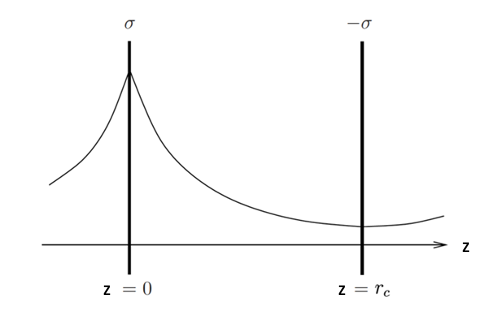
\includegraphics[scale=0.6]{Images/RS1 warp factor.png}
    \caption{A Plot of the Warp Factor in the RS1 Model showing the exponetial decay from one brane to another. $r_c$ is the distance of the second brane from the brane centered at $z=0$ \cite{Figures}.}
    \label{fig:RS1}
\end{figure}\\
\newpage
\noindent For non critical branes, $\lambda \neq 0$, we again choose to solve our first order equation of motion in the bulk. To remind ourselves, with $\lambda \neq 0$ we have
\begin{equation}
    -\Lambda+3M^3_5\left(\frac{\lambda}{a^2}-\left(\frac{a^\prime}{a}\right)^2\right)=0
\end{equation}
We take $\Lambda=-3M^3_5\kappa^2$, which leaves us with
\begin{equation}
    \kappa^2+\frac{\lambda}{a^2}=\frac{{a^\prime}^2}{a^2}
\end{equation}
We let 
\begin{equation}
    a=\frac{\sqrt{|\lambda|}}{\kappa}b
\end{equation}
so that (2.39) becomes
\begin{equation}
    \kappa^2\left[1+\frac{sign\left(\lambda\right)}{b^2}\right]=\frac{{b^\prime}^2}{b^2}
\end{equation}
Then we set 
\begin{equation}
    z=\frac{1}{\alpha}y \\
    \implies \partial_z =\kappa\partial_y
\end{equation}
Applying (2.42) to (2.41), we yield
\begin{equation}
    b^2_y=b^2\pm 1
\end{equation}
where the $\pm 1$ correspond to positive and negative cases of $\lambda $ respectively, and $b_y$ denotes the derivative of b with respect to $y$. We can rearrange (2.43) and take the integral of both sides.
\begin{equation}
    \int \frac{db}{\sqrt{b^2 \pm 1}}=\pm\int dy
\end{equation}
For $\lambda>0$, 
\begin{equation}
    \int \frac{db}{\sqrt{b^2 + 1}}=+\int dy
\end{equation}
This is a standard trigonometric integral with the result
\begin{equation}
    {sinh}^{-1}\left(b\right)+c= \pm y
\end{equation}
We recall that we defined $b=\frac{\kappa a}{\sqrt{|\lambda |}}$ and $y=\kappa z$. Substituting these back into (2.46) and rearranging for $a(z)$ we find
\begin{equation}
    a\left(z\right)=\sqrt{\frac{|\lambda |}{\kappa^2}}\sinh\left(\pm\kappa z+c\right)
\end{equation}
For $\lambda<0$, we can start from
\begin{equation}
    \int \frac{db}{\sqrt{b^2 - 1}}=\pm\int dy
\end{equation}
which is another standard integral. This becomes
\begin{equation}
    {cosh}^{-1}\left(b\right)+c=\pm y
\end{equation}
Once again recalling (2.40) and (2.42), and substituting into (2.49), we arrive at our third equation for the warp factor
\begin{equation}
 a\left(z\right)=\sqrt{\frac{|\lambda |}{\kappa^2}}\cosh\left(\pm\kappa z+c\right)
\end{equation}
We see from our work that there are three separate equations for the warp factor depending on which regime for $\lambda$ we choose.
\begin{equation}
    a\left(z\right)=
    \begin{cases}
        \sqrt{\frac{|\lambda |}{\kappa^2}}\sinh\left(\pm\kappa z+c\right)\hspace{10pt}\text{if } \lambda > 0\\[10pt]
        Ae^{\pm\kappa z}\hspace{10pt}\text{if } \lambda = 0\\[10pt]
        \sqrt{\frac{|\lambda |}{\kappa^2}}\cosh\left(\pm\kappa z+c\right) \hspace{10pt}\text{if } \lambda < 0
    \end{cases}
\end{equation}
All solutions contain $\kappa$, where $\kappa = \sqrt{\frac{-\Lambda}{3M^3_5}}$, which forces $\Lambda < 0$ to produce any real-valued functions and requires that the bulk is an $AdS_5$ spacetime.
\subsection{Calculating Brane Tensions}
We recall that by construction the Randall-Sundrum Braneworld model has $\mathbb{Z}_2$-symmetry at the domain walls $z=z_1$ and $z=z_2$ as shown in figure 2.1. The consequence of this symmetry is that it imposes the boundary conditions on the branes $a(z_1-\epsilon)=a(z_1+\epsilon)$ and $a(z_2-\epsilon) = a(z_2+\epsilon)$, which will be employed throughout the calculations that follow. We use this boundary condition and the bulk equations of motion to calculate our brane tensions in the different cases of $\lambda$.
We begin with the critical branes, $\lambda = 0$.\\
For the brane at $z=z_1$, we integrate equation (2.32) across an infinitesimal region containing $z_1$ as follows
\begin{equation}
    \int^{z_1+\epsilon}_{z_1-\epsilon}dz\left(\frac{a^{\prime\prime}}{a}+\left(\frac{a^\prime}{a}\right)^2-\frac{4\kappa^2}{M^3_5}\right)=\frac{-\sigma_1}{3M^3_5} \int^{z_1+\epsilon}_{z_1-\epsilon}dz\delta\left(z-z_1\right)-\frac{\sigma_2}{3M^3_5}\int^{z_2+\epsilon}_{z_2-\epsilon}dz\delta\left(z-z_2\right)
\end{equation}
In this range, $a(z)$ is continuous but finite, $a^\prime(z)$ is finite but not continuous and $a^{\prime\prime}(z)$ diverges on the brane. Making note of these properties it is clear that when performing the integration over this infinitesimal region, we retain only the contribution of the divergent function $a^{\prime\prime}(z)$ to get a finite answer, with all other terms being lost. We can therefore effectively rewrite our integral as
\begin{equation}
    \frac{1}{a\left(z_1\right)}\int^{z_1+\epsilon}_{z_1-\epsilon}dza^{\prime\prime}\left(z\right)=\frac{-\sigma_1}{3M^3_5} \int^{z_1+\epsilon}_{z_1-\epsilon}dz\delta\left(z-z_1\right)
\end{equation}
Which yields
\begin{equation}
    \frac{a^\prime\left(z^{+}_1\right)-a^\prime\left(z^{-}_1\right)}{a\left(z_1\right)}=\frac{-\sigma_1}{3M^3_5}
\end{equation}
Where $a^{\prime}(z_1^+) = a^{\prime}(z_1 + \epsilon)$, and corresponds to the warp factor in the infinitesimally small region $z_1+\epsilon$ and $a(z_1)$ corresponds to both the positive and negative solutions for the warp. Note that at this stage, we employ our boundary conditions and let $a(-z_1) = a(z_1)$. Then equation (2.54) becomes
\begin{equation}
    -2\kappa=\frac{-\sigma_1}{3M^3_5}
\end{equation}
We rearrange to obtain the brane tension at $z=z_1$
\begin{equation}
    \sigma_1=6\kappa M^3_5
\end{equation}
We can repeat the same process for the brane at $z=z_2$,
\begin{equation}
    \frac{1}{a\left(z_2\right)}\int^{z_2+\epsilon}_{z_2-\epsilon}dza^{\prime\prime}\left(z\right)=\frac{-\sigma_2}{3M^3_5}\int^{z_2+\epsilon}_{z_2-\epsilon}dz\delta\left(z-z_2\right)
\end{equation}
Which yields
\begin{equation}
    \frac{a^\prime\left(z^{+}_2\right)-a^\prime\left(z^{-}_2\right)}{a\left(z_2\right)}=\frac{-\sigma_2}{3M^3_5}
\end{equation}
\begin{equation}
    \implies 2\kappa=\frac{-\sigma_2}{3M^3_5}
\end{equation}
The brane tension on the second brane, $\sigma_2$, is
\begin{equation}
    \sigma_2=-6\kappa M^3_5
\end{equation}
We notice that our brane tensions have equal magnitude but are of opposite sign. Notice that the positive brane tension corresponds to the peak in $a(z)$, as seen in Figure 2.1. Recalling that $\Lambda=-3M^3_5\kappa^2$, we find a fine-tuning of the brane tensions against the Bulk Cosmological Constant, $\Lambda$. Recalling that $\Lambda=-3M^3_5\kappa^2$,
\begin{align*}
    {\sigma}^2&=\left(6\kappa M^3_5\right)^2\nonumber\\
    &=\left(6\sqrt{\frac{-\Lambda}{3M^3_5}} M^3_5\right)^2
\end{align*}
\begin{equation}
    \implies \Lambda=\frac{-\sigma^2}{12M^3_5}
\end{equation}
From equation (2.61) we can see the branes are fine-tuned against the bulk cosmological constant and that $\Lambda<0$ for all $\sigma$, again implying the Bulk is an example of an $AdS_5$ spacetime. The negative cosmological constant, $\Lambda$, prevents gravity from leaking into the bulk at low energies. The implication of this is that the RS1 model doesn't rely on compactification to localise gravity on the brane but instead on the curvature of the bulk. This is why RS1 is sometimes referred to as an alternative to compactification.\\
We now consider the non critical branes, $\lambda \neq 0$. In both cases, $\lambda > 0$ and $\lambda < 0$, we proceed in the same way as before, integrating equation (2.25) over infinitesimal regions across both branes. In both cases the only non vanishing term is still the divergent $a^{\prime\prime}(z)$. Then, for both cases, we proceed from equations (2.54) and (2.58).\\
At $z=z_1$ we have
\begin{equation}
    \frac{a^\prime\left(z^{+}_1\right)-a^\prime\left(z^{-}_1\right)}{a\left(z_1\right)}=\frac{-\sigma_1}{3M^3_5}
\end{equation}
At $z=z_2$ we have
\begin{equation}
    \frac{a^\prime\left(z^{+}_2\right)-a^\prime\left(z^{-}_2\right)}{a\left(z_2\right)}=\frac{-\sigma_2}{3M^3_5}
\end{equation}
Analysis of equations (2.62) and (2.63) gives us the following brane tensions.\\
For $\lambda > 0$,
\begin{equation}
    \sigma_1 = 6\kappa M^3_5\coth{\left(\kappa z_1 + c\right)}
\end{equation}
\begin{equation}
    \sigma_2 = -6\kappa M^3_5\coth{\left(\kappa z_2 + c\right)}
\end{equation}
For $\lambda < 0$, 
\begin{equation}
    \sigma_1 = 6\kappa M^3_5\tanh{\left(\kappa z_1 +c\right)}
\end{equation}
\begin{equation}
    \sigma_2 = 6\kappa M^3_5\tanh{\left(\kappa z_2 +c\right)}
\end{equation}
We see in both cases, the branes have opposite sign but are not necessarily of equal magnitude. Since the brane tensions may be different magnitudes, we can still find a brane tension - bulk cosmological constant relation for our non-critical branes, but we must have one relation for $\sigma_1$ and another for $\sigma_2$. We will do this by using the index $i={1,2}$ to represent $\sigma_1$ and $\sigma_2$ respectively.\\
For $\lambda > 0$, when we have De-Sitter branes we yield
\begin{equation}
    \sigma_{i}^2 = \left(6\kappa M^3_5\coth{(\kappa z_i +c)}\right)^2 
\end{equation}
Where, $\kappa = \sqrt{\frac{-\Lambda}{3M^3_5}}$. Using this, we find the relation
\begin{equation}
    \Lambda = \frac{-\sigma_i^2}{12M^3_5\coth{(\kappa z_i +c)}^2}
\end{equation}
We then see for all $\sigma_1$ and all $\sigma_2$, the brane tensions are fine tuned against the bulk cosmological constant, which is clearly negative for all $\sigma_1$, $\sigma_2$, thus forcing the bulk to be an $AdS_5$ spacetime.\\
Similarly, we can calculate this relation for our anti De-Sitter branes, $\lambda < 0$, and yield
\begin{equation}
    \Lambda = \frac{-\sigma_i^2}{12M^3_5\tanh{(\kappa z_i +c)}^2}
\end{equation}
Again, we see the bulk is an example of an $AdS_5$ spacetime for all $\sigma_1$ and all $\sigma_2$.
\subsection{Solutions}
So far we have found the form for the warp factor in the bulk for all cases of $\lambda$ and found the corresponding brane tensions. For a complete set of solutions for the warp factor, with their corresponding brane tensions, we must fix our constants of integration in the equations in (2.51), $c$ for $\lambda \neq 0$ and $A$ for $\lambda = 0$. We have the freedom to set $a(0) = 1$, allowing us to find our constants of integration. Trivially, for $\lambda = 0$ we find $A=1$.\\ For $\lambda>0$,
\begin{equation}
    \kappa = \sqrt{|\lambda|}\sinh{c}
\end{equation}
For $\lambda < 0$,
\begin{equation}
    \kappa = \sqrt{|\lambda|}\cosh{c}
\end{equation}
We can now present our solutions. Recall that $N(z)=1$.
\begin{equation}
    a\left(z\right)=
    \begin{cases}
        \sqrt{\frac{|\lambda |}{\kappa^2}}\sinh\left(\pm\kappa z+c\right)\hspace{10pt}, \kappa=\sqrt{|\lambda|}\sinh{c}\hspace{10pt}\text{if } \lambda > 0\\[10pt]
        e^{\pm\kappa z}\hspace{10pt}\text{if } \lambda = 0\\[10pt]
        \sqrt{\frac{|\lambda |}{\kappa^2}}\cosh\left(\pm\alpha z+c\right) \hspace{10pt}, \kappa=\sqrt{|\lambda|}\cosh{c}\hspace{10pt}\text{if } \lambda < 0
    \end{cases}
\end{equation}
The corresponding brane tensions are
\begin{equation}
    \sigma_1=
    \begin{cases}
         6\kappa M^3_5\coth{\left(\kappa z_1 + c\right)}\hspace{10pt}\text{if } \lambda > 0\\[10pt]
        6\kappa M^3_5\hspace{10pt}\text{if } \lambda = 0\\[10pt]
        6\kappa M^3_5\tanh{\left(\kappa z_1 +c\right)}\hspace{10pt}\text{if } \lambda < 0
    \end{cases}
\end{equation}
\begin{equation}
    \sigma_2=
    \begin{cases}
         -6\kappa M^3_5\coth{\left(\kappa z_2 + c\right)}\hspace{10pt}\text{if } \lambda > 0\\[10pt]
        -6\kappa M^3_5\hspace{10pt}\text{if } \lambda = 0\\[10pt]
        -6\kappa M^3_5\tanh{\left(\kappa z_2 +c\right)}\hspace{10pt}\text{if } \lambda < 0
    \end{cases}
\end{equation}
\subsection{A Solution to The Hierarchy Problem}
To solve the hierarchy problem, we need to derive the effective four-dimensional Planck scale in terms of our five-dimensional terms.
\\
From our derivation of the Ricci Scalar, we recall that $R = g^{zz}R_{zz} + g^{\mu\nu}R_{\mu\nu}$. We show in Appendix C that we can deconstruct the Ricci tensor into a purely four-dimensional piece and another piece that involves mixing between our four and five-dimensional coordinates, $R_{\mu\nu} = R_{\mu\nu}(q) + ...$, where the first term is our 4d piece and the rest involves mixing.\\
Consequently, we can split the Ricci scalar into four and five-dimensional terms. Recall that we set $N(z) = 1$ so that $g^{zz} = 1$.
\begin{equation}
    R = R_{zz} + \frac{1}{a^2}q^{\mu\nu}R_{\mu\nu}(q) +...
\end{equation}
\begin{equation}
    \Rightarrow R_{5}= \frac{1}{a^2}R_{4}(q) + ...
\end{equation}
where $R_5$ denotes the five-dimensional Ricci scalar and $R_4$ denotes the four-dimensional Ricci scalar.
With this result, we can separate the Einstein Hilbert action for our model into four and five-dimensional terms.
\begin{equation}
    \begin{aligned}
    S = \int dzd^4x\sqrt{-g}\frac{M^3_5}{2}R(g) = \int dza^4\sqrt{-q}\frac{M^3_5}{2}(\frac{1}{a^2}R_4(q) + ...)d^4x \\ = \int dz\sqrt{-q}a^2\frac{M^3_5}{2}(R_4(q) + ...)d^4x = (\int dza^2)\frac{M^3_5}{2}\int d^4x\sqrt{-q}R_4(q) + ...
    \end{aligned}
\end{equation}
Note, the integral on the extra dimension is unanimous with the volume element for the extra dimension. This is important since the effective four dimensional Planck Scale, $M_{PL}$, is determined by the five dimensional Planck Scale, $M^3_5$, and the volume of the the fifth dimensional space \cite{RS1}, $V_n$, by the relation 
\begin{equation}
    M_{PL}^{2} = M^2_4 = M_{5}^3V_n 
\end{equation}
where we have identified
\begin{equation}
    V_n = \int dza^2
\end{equation}
Before progressing further, we refer back to figure 2.1 and define three distinct regions, regions 1,2 and 3. Region 1 is the space $z<z_1$, region 2 is the space $z_1<z<z_2$ and region 3 is the space $z>z_2$.\\
We can substitute (2.80) back into equation (2.79), and perform an integral over regions 1 and 2.
\begin{equation}
    M^2_4 = M_5^3V_n = M^3_5\int^{z_1 + r_c}_{z_1 - r_c}dza^2
\end{equation}
Where $a^2 = e^{\pm2kz}$, depending on the region. We also remind ourselves the extrinsic curvature, $\lambda$, is zero. Equation (2.81) becomes
\begin{equation}
    \begin{aligned}
        M^2_4 = M^3_5(\int^{z_1 + r_c}_{z_1}dze^{-2\kappa z} + \int^{z_1}_{z_1 - r_c}dze^{2\kappa z}) \\
        = M^3_5\frac{1}{2\kappa}[-e^{-2\kappa(z_1+r_c)}+e^{-2\kappa z_1}+e^{-2\kappa z_1}-e^{2\kappa (z_1 -r_c)}] \\
        = M^3_5\frac{1}{2\kappa}[2e^{2\kappa z_1} -2e^{2\kappa z_1}e^{-2\kappa r_c}]
    \end{aligned}
\end{equation}
where in the last line we use the continuity conditions on the brane that $e^{-2\kappa z_1} = e^{2\kappa z_1} = a^2(z_1)$.

\begin{equation}
    \begin{aligned}
        \Rightarrow M^2_4 = M^3_5\frac{1}{2\kappa}[2a^2(z_1) - 2a^2(z_1)e^{-2\kappa r_c}]= M^3_5\frac{1}{2\kappa}2a^2(z_1)[1-e^{-2\kappa r_C}]
    \end{aligned}
\end{equation}
Then, we reach our final result and the four dimensional effective Planck scale is
\begin{equation}
     M^2_4 = M^3_5\frac{a^2(z_1)}{\kappa}[1-e^{-2\kappa r_c}]
\end{equation}
where if we set $z_1 = 0$ and allow $a(0)=1$ we have
\begin{equation}
     M^2_4 = \frac{M^3_5}{\kappa}[1-e^{-2\kappa r_c}]
\end{equation}
It can also be shown that an observer on the brane will measure the Higgs mass to be
\begin{equation}
    m_H = e^{-\kappa r_c}m_0
\end{equation}
where $m_0$ is the fundamental Higgs mass \cite{padilla2002braneworld}.
If the fundamental Planck scale, $M^3_5$, and the fundamental Higgs mass, $m_0$, are both of order $10^{18}$ GeV, we have no hierarchy in the five dimensional theory. The effective theory, as seen by an observer on the brane, will yield values of the Higgs mass, $m_H$, and the Planck scale, $M^2_4$, controlled by the equations (2.85) and (2.86). The effective theory then is able to make predictions consistent with observation through a rescaling of our fundamental values via the warp factor, where the extent of the rescaling depends on $\kappa r_c$. Consequently, our ability to produce a viable solution is intimately linked to the brane seperation $r_c$. If the fundamental Planck scale and the fundamental Higgs mass are both of order $10^{18}$GeV, we see we require $e^{\kappa r_c} \approx 10^{15}$ to ensure that $m_H \approx 10^3$GeV and $M_4 \approx 10^{18}$GeV, as observed in nature \cite{padilla2002braneworld}. Alternatively, we could take the opposite approach and set the fundamental Higgs mass and the fundamental Planck mass to be much smaller, as long as they are both set to the same scale, and reproduce the correct effective theory. The RS1 model is able to provide a solution to the hierarchy problem without the need for the extra dimension to be large and therefore doesn't introduce new hierarchies between the weak scale and the compactification scale, unlike many other proposed solutions. 
\section{RS2}
Since all Standard Model fields are bound to the brane, we must be able to reproduce Newtons laws on the brane. Previous braneworld models achieve this by constraining the extra dimension to be small and compact. The RS2 model removes this constraint, and is able to reproduce Newtons laws on the brane despite having an infinite extra dimension. Gravity is localised on the brane due to the curvature of our $AdS_5$ bulk, allowing us the freedom to extend the extra dimension to infinity whilst remaining consistent with Newtons laws on the brane. The RS2 model is no longer concerned with the hierarchy problem, so we sacrifice our solution to the hierarchy problem to remove the constraint set on the size of the extra dimension.\\
We begin with the familiar RS1 model and sending the negative tension brane to infinity, $z_2 \longrightarrow \infty$. We are left with an infinite bulk and a single brane with positive tension at $z = 0$, embedded in $AdS_5$ space. The standard model fields are bound to the remaining brane, so that in this model we exist as observers on the brane with positive tension rather than the brane with negative tension as in the RS1 model.
Our metric remains the same as in equation (2.1), to remind ourselves we have
\begin{equation}
    ds^2= N^2(z)dz^{2} + a^{2}(z) q _{\mu\nu}(x) dx^{\mu} dx^{\nu}
\end{equation}
where before we found, in the bulk for $\lambda = 0$, $a(z) = e^{-\kappa z}$ and $N(z)=1$. Then equation (2.87) becomes
\begin{equation}
    ds^2= dz^{2} + e^{-2\kappa z}q _{\mu\nu}(x) dx^{\mu} dx^{\nu}
\end{equation}
We can represent the behaviour of the warp factor in the RS2 model graphically as in Figure 2.2. 
\begin{figure}[H]
\centering
    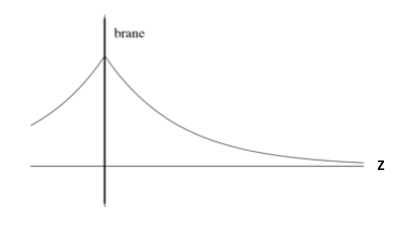
\includegraphics[scale=0.8]{Images/RS2 model.png}
    \caption{Behaviour of the Warp Factor in the RS2 Model, with a single brane of positive tension at $z=0$ \cite{Figures}.}
    \label{fig:RS2}
\end{figure}
\noindent The RS2 model may not be a viable phenomenology when combined with bimetric gravity, since two branes are needed to support a braneworld bi-gravity set-up \cite{Kaloper:2018dqn}. In this paper, we choose to proceed with the RS1 model for this reason. Despite this, if a viable solution is found using an RS1 set-up, it could be of interest to see what results an RS2 model would yield since Randall -Sundrum bimetric theories have not been explored. 

\chapter{Massive Gravity}
\section{Non-Trivially Interacting Massless Helicity 2-Particles}
Without Einstein's leap of insight, the discovery of General relativity would likely have been delayed several decades until advancements in field theory would allow field theorists of the 1940s / 1950s to arrive at general relativity.
While Einstein and the field theorists would derive the same general relativity, their approaches would be drastically different. In many ways, field theorists' path to general relativity would be far more logical and lead uniquely to general relativity. Einstein's approach was not a logical one; general coordinate invariance and the equivalence principle were the insights that led Einstein to general relativity, but both general coordinate invariance and the equivalence principle are not fundamental properties of general relativity and do not lead uniquely to general relativity. In fact, we can make any Lagrangian invariant under general coordinate diffeomorphisms through the Stuckelberg trick.
The most accurate way to define general relativity is as the theory of a non-trivially interacting massless helicity 2 particle, the graviton. This statement is the foundation of the field theorist's approach. 
Field theory tells us that in a Minkowski spacetime, degrees of freedom are particles that are represented and carried by fields, defined by their spin. Long-range forces are carried by massless bosonic fields of integer spin, $m=0$. We can characterize massless particles by their helicity. For a helicity 2 particle, general coordinate invariance is the required gauge symmetry to produce a theory with consistent self-interactions. It is important to realise that general coordinate invariance is a gauge symmetry and not a fundamental property of general relativity. We can always eliminate gauge symmetries by fixing the gauge and we can create gauge symmetries through the Stuckelberg trick. This discussion of gauge symmetries will become important when we consider theories of massive gravity and the naturalness of solutions to such theories.

\section{Introduction to Massive Gravity}
Since General Relativity is the theory of a non-trivially interacting massless helicity 2 particle, the first obvious deformation we can consider is to disregard the massless condition and give mass to the graviton. The first to develop a model of massive gravity was Fierz and Pauli who, in 1939, derived the Fierz -Pauli action\cite{fierz1939relativistic}
\begin{equation}
    S = \int d^4 x- \frac{1}{2}\partial_{\lambda}h_{\mu\nu}\partial^{\lambda}h^{\mu\nu} + \partial_{\mu}h_{\nu\lambda}\partial^{\nu}h^{\mu\lambda} -\partial_{\mu}h^{\mu\nu}\partial_{\nu}h +\frac{1}{2}\partial_{\lambda}h\partial^{\lambda}h - \frac{1}{2}m^2\left(h_{\mu\nu}h^{\mu\nu}-h^2\right)
\end{equation}
that models a Lorentz invariant, non-self-interacting, massive spin-2 particle that propagates on a flat Minkowski background. Following this however, developments in the field stalled until around the 1970s when, during the resurgence of quantum field theory, van Dam, Veltman and Zarkharov showed how the model diverged significantly from the predictions of gravitational lensing around massive objects in general relativity\cite{Kurts_review}. These predictions differed by as much as 25\% and were due to the fact that massive spin-2 fields propagate with 5 degrees of freedom regardless of the size of the mass\cite{de_Rham_2014} as they do not decouple. Since general relativity is a theory with only two propagating degrees of freedom\cite{de_Rham_2014}, it seems that massive gravity cannot be compatible with it, even in the $m \longrightarrow 0$ limit. This pathology became known as the vDVZ discontinuity\cite{Kurts_review}. \\
Fortunately, a way to circumvent the vDVS discontinuity was found via the Vainshtein mechanism only a short while after which argues that the discontinuity belongs only to the linear theory and can be resolved by invoking higher order terms\cite{VAINSHTEIN1972393} \cite{Babichev_2013}. Vainshtein discovered that in the vicinity of large objects, a distance from that object known as the Vainshtein radius can be identified beyond which non-linearities dominate the lower order terms meaning the vDVZ discontinuity gives way. 
\begin{equation}
    r_v \sim \left(\frac{M}{m^4M^2_{PL}}\right)
\end{equation}
Here $r_v$ is the Vainshtein radius and $m$, $M$ and $M_{PL}$ are the masses of the graviton and large object respectively and  is the Planck mass. It was shown also that in the massless limit $m \longrightarrow 0$, the Vainshtein radius, $r_v$ goes to infinity and the vDVZ is removed from the theory\cite{Kurts_review}. This period of an apparent resolution was short-lived however and soon yet another problem was discovered when transitioning to fully non-linear theories that comprise interactions with the standard model. Issues were already encountered with 5 degrees of freedom and yet the non-linear extensions studied by Bouleware and Deser were found to propagate with 6, where this $6^{th}$ extra degree takes the form of a scalar field with a negative kinetic term, later named as the Boulewere-Deser ghost\cite{BDGhost}. \\
Eliminating the extra degree of freedom in the non-linear theory is essential to avoiding the Boulewere-Deser ghost and Massive gravity was the subject of significant interest when recently deRham, Gababadaze and Tolley published a solution\cite{de_Rham_2010}. They proposed the most general form of a potential that can be added to an Einstein-Hilbert kinetic term which constrains the interaction terms in such a way that reduces the total degrees of freedom of the theory and eradicates the extra scalar degree of freedom belonging to the Boulware-Deser ghost\cite{de_Rham_2010}\cite{de_Rham_2011}\cite{Kurts_review}. The theory raises the energy cutoff of the effective theory, at which point the ghost is removed. The resulting ghost-free theories are known as dRGT theories of massive gravity and they can be written as\cite{BDHinterbichler_2013},
\begin{equation}
    S=\frac{M_{PL}^2}{2}\int d^4x \sqrt{-g}\left[R-\frac{m^2}{2}\sum^4_{n=0}\beta_n S_n \left(\sqrt{g^{-1}\eta}\right)\right]
\end{equation}
In this paper, our interest in massive gravity is due to its link to the Cosmological Constant problem, which we recall as the discrepancy between the observed value of the constant measured from observations of the expansion of the universe and the value predicted from vacuum fluctuations in quantum field theory. Massive gravity provides potential solutions to the problem through the degravitation method. This is a modification where the mass of the graviton acts as a filtering scale in the coupling of gravity to the cosmological constant\cite{CCMassive}. This effectively shifts the question from why the constant has such a small magnitude to instead why it gravitates so little, which we are better prepared to answer and exact details can be found in\cite{BigravCC}.

\section{Multi-Metric Models}
Multi-metric theory is a generalisation of the Einstein-Hilbert kinetic term to N, initially non-interacting, spin-2 fields with each having an associated metric, Planck mass, and cosmological constant which we can be written as the summation\cite{Hinterbichler:2012cn}
\begin{equation}
    \mathcal{L} = \sum_{I=1}^N \frac{M_I^{D-2}}{2}\sqrt{-g_{(I)}} ( R(g_{(I)})-2\Lambda_(I))
\end{equation}
To capture the interactions between multiple metrics, Hinterbichler and Rosen derived  a generalisation of the dRGT ghost-free theory for a single massive graviton in \cite{Hinterbichler:2012cn}, and produced an interaction term for $N$ interacting spin-2 fields in D-dimensions.
\begin{equation}
U=\sum^N_{I_1I_2...I_D=1}T^{I_1I_2...I_D}\Tilde{\epsilon}_{A_1A_2...A_D}\bold{E}_{I_1}^{A_1}\wedge\bold{E}_{I_2}^{A_2}\wedge ...\wedge\bold{E}_{I_D}^{A_D}
\end{equation}
Here $T$ is a symmetric tensor of coefficients and $\Tilde{\epsilon}$ is the anti-symmetric epsilon symbol. This form is far easier to work with than the traditional dRGT potential which uses matrix square roots. Hinterbickler and Rosen's term has a veilbein structure instead which is intuitive as vielbeins can be interpreted as the square root of a metric. Each metric has a vielbein one-form\cite{Kurts_review}, 
\begin{equation} 
\bold{E}^A_I = E^A_{I_\mu}(x)dx^\mu
\end{equation}
that relates it back to the flat metric, 
\begin{equation}
    g_{(I)_{\mu\nu}} = E^A_{I_\mu}E^B_{I_\nu}\eta_{AB}
\end{equation}
For a theory with only one metric, our potential will only have one term, whereas a bi-metric theory has two metrics and will have $D-1$ terms that we have to find which mix between the components of the two metrics. In fact, we can see that for arbitrary dimension, $D$, with $N$ interacting metrics, we can write the total number of unique terms as $\binom{N+D-1}{D}$ and the if the number of metrics exceeds the number of dimensions then we can say there exist no terms that mix terms from all metrics in the system\cite{Kurts_review}. Combining this potential with (3.4) forms the action,
\begin{equation}
    S = \int dzd^4x\sum_{I=1}^N \frac{M_I^{D-2}}{2}\sqrt{-g_{(I)}}(R(g_{(I)})-2\Lambda_(I)) + \sum^N_{I_1,I_2,...,I_D} T^{I_1I_2...I_D}\Tilde{\epsilon}_{A_1A_2...A_D}\bold{E}_{I_1}^{A_1}\wedge\bold{E}_{I_2}^{A_2}\wedge ...\wedge\bold{E}_{I_D}^{A_D}
\end{equation}
\section{Bimetric Theory}
Having started from the action of a Multi-Metric system, we can now specify from the general form the specific number of Gravitons we want to include in our system as well as the number of dimensions we wish to work in. This paper will study a Bimetric system with two Gravitons and, as we are attempting to combine this with the RS1 regime, we will specify 5 spacetime dimensions. Using the dRGT interaction term, our action for this model is\cite{Hinterbichler:2012cn},
\begin{align}
    S = \int dzd^4x\frac{M_1^{3}}{2}\sqrt{-g_{(1)}}(R(g_{(1)})-2\Lambda_{(1)}) + \frac{M_2^{3}}{2}\sqrt{-g_{(2)}}(R(g_{(2)})-2\Lambda_{(2)})\\ \nonumber+\sum^N_{I_1I_2...I_5}T^{I_1I_2...I_5}\Tilde{\epsilon}_{A_1A_2...A_5}\bold{E}_{I_1}^{A_1}\wedge\bold{E}_{I_2}^{A_2}\wedge ...\wedge\bold{E}_{I_5}^{A_5}
\end{align}
We now have to find the explicit form of our interaction terms. To do this we will use the metric we defined previously (2.1) and use it to write a basis of 1-forms for our system $E^z_i$ and $E^\alpha_i$,
\begin{equation}
ds^2_i=N^2_i\left(z\right)dz^2+a^2_i\left(z\right)q_{\mu\nu}\left(x\right)dx^\mu dx^\nu
\end{equation}
\begin{equation}
    E^z_i=N_idz 
\end{equation}
\begin{equation}
    E^\alpha_i=a_ie^\alpha 
\end{equation}
\begin{equation}
    q_{\mu\nu}dx^\mu dx^\nu=\eta_{\alpha \beta}e^\alpha \otimes e^\beta
\end{equation}
where $q_{\mu\nu}$ is maximally symmetric metric on the branes with curvature $\lambda$.\\

Using the interaction term (3.5), we can write out the form of the interaction term for our model as,
\begin{align}
    U=T^{11111}E^{a_1}_1\wedge E^{a_2}_1\wedge E^{a_3}_1\wedge E^{a_4}_1\wedge E^{a_5}_1\Tilde{\epsilon}_{a_1...a_5}\\ \nonumber
    +T^{11112}E^{a_1}_1\wedge E^{a_2}_1\wedge E^{a_3}_1\wedge E^{a_4}_1\wedge E^{a_5}_2 \Tilde{\epsilon}_{a_1...a_5}\\ \nonumber
    +T^{11122}E^{a_1}_1\wedge E^{a_2}_1\wedge E^{a_3}_1\wedge E^{a_4}_2\wedge E^{a_5}_2\Tilde{\epsilon}_{a_1...a_5}\\ \nonumber
    +T^{11222}E^{a_1}_1\wedge E^{a_2}_1\wedge E^{a_3}_2\wedge E^{a_4}_2\wedge E^{a_5}_2\Tilde{\epsilon}_{a_1...a_5}\\ \nonumber
    +T^{12222}E^{a_1}_1\wedge E^{a_2}_2\wedge E^{a_3}_2\wedge E^{a_4}_2\wedge E^{a_5}_2\Tilde{\epsilon}_{a_1...a_5}\\ \nonumber
    +T^{22222}E^{a_1}_2\wedge E^{a_2}_2\wedge E^{a_3}_2\wedge E^{a_4}_2\wedge E^{a_5}_2\Tilde{\epsilon}_{a_1...a_5} \nonumber
\end{align}
Let us look deeper at the first term,
\begin{equation}
    T^{11111}E^{a_1}_1\wedge E^{a_2}_1\wedge E^{a_3}_1\wedge E^{a_4}_1\wedge E^{a_5}_1\epsilon_{a_1...a_5}
\end{equation}
Using the properties of the Levi-Civita symbol and that 
\begin{equation}
    \epsilon^{i_1...i_n}\epsilon_{i_1...i_n}=n!
\end{equation}
We can rewrite this as
\begin{equation}
    =5!T^{11111}E^{1}_1\wedge E^{2}_1\wedge E^{3}_1\wedge E^{4}_1\wedge E^{5}_1
\end{equation}
and again using (3.11) and (3.12),
\begin{equation}
    =5!T^{11111}N_1a_1^4dze^{2}\wedge e^{3}\wedge e^{4}\wedge e^{5}
\end{equation}
If write our 4 dimensional metric $q_{\mu\nu}$ as
\begin{equation}
    q_{\mu\nu}=\frac{\partial e^\alpha}{\partial x^\mu}\eta_{\alpha\beta}\frac{\partial e^\beta}{\partial x^\nu}
\end{equation}
then we can take the determinant of each side,
\begin{equation}
     det\left(q\right)=\left|\frac{\partial e^\alpha}{\partial x^\mu}\right|det\left(\eta\right)\left|\frac{\partial e^\beta}{\partial x^\nu}\right|
\end{equation}
and since $det\left(\eta\right)=-1$,
\begin{equation}
    det\left(q\right)=-\left|\frac{\partial e^\alpha}{\partial x^\mu}\right|^2
\end{equation}
Thus we can write a jacobian for the transformation between 1-forms and volume elements
\begin{equation}
    J=\sqrt{-q}
\end{equation}
Using this we can rewrite the wedge product as, 
\begin{equation}
    e^{2}\wedge e^{3}\wedge e^{4}\wedge e^{5}=\sqrt{-q}dx^{2}\wedge dx^{3}\wedge dx^{4}\wedge dx^{5}
\end{equation}
and so
\begin{equation}
    5!T^{11111}N_1a_1^4dze^{2}\wedge e^{3}\wedge e^{4}\wedge e^{5}=5!T^{11111}N_1a_1^4\sqrt{-q}dzd^4x
\end{equation}
which is an explicit form for this term.\\
We proceed via a similar process for the remaining terms to arrive at our complete interaction term,
\begin{align}
    U&=5!T^{11111}N_1a_1^4\sqrt{-q}dzd^4x\\ \nonumber
     &+5!T^{11112}\left(4N_1a_1^3a_2+N_2a_1^4\right)\sqrt{-q}dzd^4x\\ \nonumber
     &+2\cdot5!T^{11122}\left(3N_1a_1^2a_2^2+2N_2a_2a_1^3\right)\sqrt{-q}dzd^4x\\ \nonumber
     &+2\cdot5!T^{11222}\left(2N_1a_1a^3_2+3N_2a_1^2a_2^2\right)\sqrt{-q}dzd^4x\\ \nonumber
     &+5!T^{12222}\left(N_1a_2^4+4N_2a_2^3a_1\right)\sqrt{-q}dzd^4x\\ \nonumber
     &+5!T^{22222}\left(N_2a_2^4\right)\sqrt{-q}dzd^4x\\ \nonumber
\end{align}
We can see that the interaction term introduces two new cosmological constant terms that do not mix metrics and have symmetric tensor coefficients $T^{11111}$  and $T^{22222}$. We can get rid of these redundancies by redefining our symmetric tensor coefficients as
\begin{equation}
    T^{11111}+\frac{2\Lambda_1}{5!} \longrightarrow T^{11111}
\end{equation}
\begin{equation}
    T^{22222}+\frac{2\Lambda_2}{5!} \longrightarrow T^{22222}
\end{equation}
\begin{align}
    S&=\int dzd^4x\frac{M_1^{3}}{2}N_1a_1^4\sqrt{-q}R(g_{(1)})+ \frac{M_2^{3}}{2}N_2a_2^4\sqrt{-q}R(g_{(2)})\\ \nonumber
    &+5!T^{11111}N_1a_1^4\sqrt{-q}\\ \nonumber
    &+5!T^{11112}\left(4N_1a_1^3a_2+N_2a_1^4\right)\sqrt{-q}\\ \nonumber
    &+2\cdot5!T^{11122}\left(3N_1a_1^2a_2^2+2N_2a_2a_1^3\right)\sqrt{-q}\\ \nonumber
    &+2\cdot5!T^{11222}\left(2N_1a_1a^3_2+3N_2a_1^2a_2^2\right)\sqrt{-q}\\ \nonumber
    &+5!T^{12222}\left(N_1a_2^4+4N_2a_2^3a_1\right)\sqrt{-q}\\ \nonumber
    &+5!T^{22222}N_2a_2^4\sqrt{-q} 
\end{align}
 Alongside the dRGT potential, there is a second constraint we must impose on the model if we wish to avoid ghost instabilities when coupling to matter. Hassan, Schmidt-May and Von Strauss showed in 2012 that we can only couple one metric to matter for the system to be stable\cite{Hassan:2012wr}, hence we will need to decouple one of our two metrics and the graviton it corresponds to such that it will not be dynamic. We will choose to couple $g_1$ only and to do this we will send $M_2^{3}$ to infinity and, as the Planck mass is proportional to $\frac{1}{G}$, where $G$ is Einstein's gravitational constant, also send $G$ to zero. This can be thought of as being analogous to "switching off" gravity and effectively fixes the values of the metric $g_2$ to be non-dynamical and Minkowski. In fact, as a consequence of this decision,
\begin{equation}
    N_2\left(z\right)=1,
\end{equation}
\begin{equation}
    a_2\left(z\right)=1
\end{equation}
and we can show that $g_1$ and $g_2$ correspond to a massive and massless graviton respectively\cite{Kurts_review}. For an overview of this, we start from the theory of two metrics with canonical kinetic terms, here in 4 dimensions for simplicity, and some potential to capture the interactions between them
\begin{equation}
    \mathcal{L}=M_1^2 R_1\sqrt{-g_1}+M_2^2 R_2\sqrt{-g_2} - V\left(g_1,g_2\right)
\end{equation}
supposing we have vacuum solutions to theory, which we will take here to be Minkowski (again for simplicity), with some perturbations $h_{\mu\nu}^{(1)}$ and $h_{\mu\nu}^{(2)}$,
\begin{equation}
    g_{\mu\nu}^{(1)}=\eta_{\mu\nu}+h_{\mu\nu}^{(1)}
\end{equation}
\begin{equation}
    g_{\mu\nu}^{(2)}=\eta_{\mu\nu}+h_{\mu\nu}^{(2)}
\end{equation}
We can then insert these solutions back into our Lagrangian and then, expanding in our perturbations take the leading order corrections to write down a quadratic order action in, $h_{\mu\nu}^{(1)}$, 
\begin{align}
    S&=\int d^4 x -\frac{1}{2}\partial_{\lambda}\tilde{h}_{\mu\nu}^{(0)}\partial^{\lambda}\tilde{h}^{\mu\nu}_{(0)}+\partial_{\mu}\tilde{h}_{\nu\lambda}^{(0)}\partial^{\nu}\tilde{h}^{\mu\lambda}_{(0)} -\partial_{\mu}\tilde{h}^{\mu\nu}_{(0)}\partial_{\nu}\tilde{h}^{(0)} +\frac{1}{2}\partial_{\lambda}\tilde{h}^{(0)}\partial^{\lambda}\tilde{h}^{(0)} \\ \nonumber
    &-\frac{1}{2}\partial_{\lambda}\tilde{h}_{\mu\nu}^{(m)}\partial^{\lambda}\tilde{h}^{\mu\nu}_{(m)}+\partial_{\mu}\tilde{h}_{\nu\lambda}^{(m)}\partial^{\nu}\tilde{h}^{\mu\lambda}_{(m)}-\partial_{\mu}\tilde{h}^{\mu\nu}_{(m)}\partial_{\nu}\tilde{h}^{(m)} +\frac{1}{2}\partial_{\lambda}\tilde{h}^{(m)}\partial^{\lambda}\tilde{h}^{(m)}-\frac{1}{2}m^2\left(\tilde{h}_{\mu\nu}^{(m)}\tilde{h}^{\mu\nu}_{(m)}-\tilde{h}_{(m)}^2\right)
\end{align}
This action includes all possible tensor contractions of two powers of $h$, that have up to two derivatives\cite{Kurts_review} and is known as the GR action to quadratic action. We can see that $h^{(m)}$ possesses a term that the $h^{(0)}$ does not, the Pauli-Fierz mass term. We see the field count remains the same however instead of $h^{(1)}$ and $h^{(2)}$ we instead have $h^{(0)}$ and $h^{(m)}$, which are associated with massless and massive gravitons respectively. The terms do not correspond directly and instead are identified, with higher order terms omitted, as
\begin{equation}
    \tilde{h}^{(0)}_{\mu\nu}=\alpha h^{(1)}_{\mu\nu} + \beta h^{(2)}_{\mu\nu} + \dots
\end{equation}
\begin{equation}
    \tilde{h}^{(m)}_{\mu\nu}=\gamma h^{(1)}_{\mu\nu} + \sigma h^{(2)}_{\mu\nu}+\dots
\end{equation}
with the particular combination contingent on coefficients which are themselves dependent on the two Planck masses $M_1$ and $M_2$. In the limit of sending $M_2$ to infinity, that we have introduced to decouple our second metric, the coefficients are evaluated such that the massive graviton is entirely comprised of $g_1$ terms and likewise $g_2$ for the massless. Precise details on this process can be found in \cite{Kurts_review}. Applying this decoupling and so (3.29) and (3.30), we are left with only $g_1$ terms,
\begin{align}
    S&=\int dzd^4x\frac{M_1^{3}}{2}N_1a_1^4\sqrt{-q}R(g_{(1)})+ \\ \nonumber
     &+5!T^{11111}N_1a_1^4\sqrt{-q}\\ \nonumber
     &+5!T^{11112}\left(4N_1a_1^3+a_1^4\right)\sqrt{-q}\\ \nonumber
     &+2\cdot5!T^{11122}\left(3N_1a_1^2+2a_1^3\right)\sqrt{-q}\\ \nonumber
     &+2\cdot5!T^{11222}\left(2N_1a_1+3a_1^2\right)\sqrt{-q}\\ \nonumber
     &+5!T^{12222}\left(N_1a+4a_1\right)\sqrt{-q}\\ \nonumber
     &+5!T^{22222}N_2a_2^4\sqrt{-q}\\ \nonumber
\end{align}
This is a model of Bimetric massive gravity in 5 dimensions.

\chapter{Constructing Bimetric Gravity in Randall-Sundrum}
We have now laid out all the necessary frameworks for us to proceed with incorporating Bimetric Gravity into the RS1 model. As this is now in the RS1 model we can reintroduce our branes back into the action. We will first look at the non-interacting case and then attempt to introduce the interactions through perturbations of these solutions. \\
For the non-interacting case, we choose to neglect, for now, any interaction terms in our model.
\begin{align}
    S=\int dzd^4x\frac{M_1^{3}}{2}&N_1a_1^4\sqrt{-q}\left(R(g_{(1)})-2\Lambda _2\right)+ \frac{M_2^{3}}{2}N_2a_2^4\sqrt{-q}\left(R(g_{(2)})-2\Lambda _2\right)\\
    &-N_1a_1^4\sqrt{-q}\left(\sigma_1(z)\delta\big(z-z_1\big)+\sigma_2\delta\big(z-z_2\big)\right)
\end{align}
When we derive equations of motion for this we reproduce our equations of motion for the RS1 model, where we have a redefined cosmological constant $\Lambda_1$ and all $a$ terms and $N$ terms belong to metric 1. 
\begin{equation}
-2\Lambda_1+3M_5^3\bigg\{\frac{\lambda}{a^2}-\bigg(\frac{a^\prime}{a}\bigg)^2\frac{1}{N}+\frac{N^\prime}{N^3}\bigg(\frac{a^\prime}{a}\bigg)-\frac{1}{N^2}\left(\frac{a^{\prime\prime}}{a}\right)\bigg\}=\\
\sigma_1a^3(z)\delta\big(z-z_1\big)+\sigma_2a^3(z)\delta\big(z-z_2\big)
\end{equation}
\begin{equation}
     -\Lambda_1++3M^3_5\left(\frac{\lambda}{a^2}-\frac{1}{N^2}\left(\frac{a^\prime}{a}\right)^2\right)=0
\end{equation}
These solutions were derived previously in Chapter 2 and by adding them to the fixed second metric solutions we have,\\
\begin{equation}
    a_1\left(z\right)=
    \begin{cases}
        \sqrt{\frac{|\lambda |}{\kappa^2}}\sinh\left(\pm\kappa z+c\right)\hspace{10pt}\text{if } \lambda > 0\\[10pt]
        Ae^{\pm\kappa z}\hspace{10pt}\text{if } \lambda = 0\\[10pt]
        \sqrt{\frac{|\lambda |}{\kappa^2}}\cosh\left(\pm\kappa z+c\right) \hspace{10pt}\text{if } \lambda < 0
    \end{cases}
\end{equation}
With $N_1(z)$, $N_2(z)$ and $a_2(z)$ equal to zero for all cases under our chosen constraints and $\kappa = \sqrt{\frac{-\Lambda_1}{3M^3_5}}$ with our redefined cosmological constant term.
\section{Background Solutions}
Now that we have our solutions we can now attempt to derive our background solutions for the complete model. We choose to do this, not analytically, but rather by introducing the mixing terms through first-order perturbations of our non-interacting solutions as seen below.
\begin{equation}
\begin{aligned}[c]
    a_1\left(z\right)&=\Bar{a}+\epsilon\delta a_1 \hspace{1cm}\\
    a_2\left(z\right)&=1  +\epsilon\delta a_2
\end{aligned}
\begin{aligned}[c]
    N_1\left(z\right)&=1 \hspace{1cm}\\
    N_2\left(z\right)&=1+\epsilon\delta N_2
\end{aligned}
\end{equation}
where $\Bar{a}_1$ is our non-interacting case solution and $\delta$ terms are our perturbations of order epsilon. Now that now we are considering the interacting case that includes mixing terms it is essential that we recognise the subtly which means we can now only choose a value for $N_1(z)=1$. To understand why, consider the coordinate transformation we applied to our metric in Chapter 2.1.2,
\begin{equation}
    z\xrightarrow{}f(z)
\end{equation}
\begin{equation}
    ds^2=N^{2}(f(z)){f^\prime}^2 dz^{2} + a^{2}(f(z)) q_{\mu\nu}(x) dx^{\mu} dx^{\nu}\\   
\end{equation}
We can see that $a(z)$ exhibits gauge invariance and can also deduce that $\frac{N_1}{N_2}$ does as well. In bigravity, there are two diffeomorphisms, one for each metric, however, when we couple them through interaction terms this is reduced to a single copy. We used $N(z)$'s lack of gauge invariance previously to fix the value $N_1\left(z\right)=1$, however, as $\frac{N_1}{N_2}$ is also gauge invariant if $N_1$ is fixed then we no longer have the freedom to fix $N_2$. With this in mind, our action becomes
\begin{align}
    S=\int dzd^4x\frac{M_1^{3}}{2}&a_1^4\sqrt{-q}R(g_{(1)})+ \frac{M_2^{3}}{2}N_2a_2^4\sqrt{-q}R(g_{(2)})\\ \nonumber
    &-N_1a_1^4\sqrt{-q}\left(\sigma_1(z)\delta\big(z-z_1\big)+\sigma_2\delta\big(z-z_2\big)\right)\\ \nonumber
    &+5!T^{11111}N_1a_1^4\sqrt{-q}\\ \nonumber
    &+5!T^{11112}\left(4a_1^3a_2+N_2a_1^4\right)\sqrt{-q}\\ \nonumber
    &+2\cdot5!T^{11122}\left(3a_1^2a_2^2+2N_2a_2a_1^3\right)\sqrt{-q}\\ \nonumber
    &+2\cdot5!T^{11222}\left(2a_1a^3_2+3N_2a_1^2a_2^2\right)\sqrt{-q}\\ \nonumber
    &+5!T^{12222}\left(a_2^4+4N_2a_2^3a_1\right)\sqrt{-q}\\ \nonumber
    &+5!T^{22222}N_2a_2^4\sqrt{-q}\\ \nonumber
\end{align}
To derive a perturbative solution our approach is to find a mtrix equation as follows

\begin{equation}
    \underline{\underline M} \hspace{0.1cm}\underline{u}^{\prime} +\underline{\underline A} \hspace{0.1cm} \underline u=\underline{v}(z)
\end{equation}
where $\underline{\underline M}$ and $\underline{\underline A}$ are matrices containing coefficients of our perturbation terms, $\underline{v}(z)$ corresponds to our $T^{mixing}$ terms and 
\begin{align}
    \underline{u}= \begin{bmatrix}
           \delta a_{1} \\
           \delta a_{2} \\
           \delta N_{2}
         \end{bmatrix}
    \hspace{1cm}
    \underline{u}^{\prime}= \begin{bmatrix}
           \delta a_{1}^{\prime}  \\
           \delta a_{2}^{\prime}  \\
           \delta N_{2}^{\prime} 
         \end{bmatrix}
\end{align}
We suspect a matrix equation of this form could be found by deriving the three possible equations of motion, for $a_1(z)$, $a_2(z)$ and $N_2(z)$. There will be no equation of motion for $N_1(z)$ as it is still in the background, $N_1(z)=1$, as in (4.6). The next step after deriving the equations of motion would be to consider the individual terms that comprise them. Substitution of our perturbed background solutions, equations (4.6), into our equations of motion and subtracting the original background equation of motion would yield the perturbation of the equations of motion. It is important to remember that our $T^{(mixing)}$ terms correspond to perturbations themselves and the product of the mixing terms with any $\delta a$'s or $\delta N$'s would produce perturbations of quadratic order, which we take to be small and would vanish. Then we suspect terms that include products between the $T^{mixing}$ terms and $a_1$, $a_2$ or $N_2$, would reduce to the product of the mixing terms and the background solutions, i.e $T^{mixing}a_1(z)$ would yield $T^{mixing} \Bar{a_1(z)}$ and would still be a perturbation term since the mixing term corresponds to a first-order perturbation.

Each equation of motion, once perturbed and after subtracting the background equation, would then represent the difference in the equations of motion and, hopefully, be a linear expression of new $T^{mixing}$ terms (potentially with $z$ dependence) and the components of the vectors $\underline{u}$ and $\underline{u^{\prime}}$. We would then have three euqations of motion and three unknown variables. This would be a linear system of ordinary differential equations as in (4.10) which we can use Green's functions to solve. 

\chapter{Discussion}
The model we have derived in the final chapter of our paper could present a potentially interesting phenomenology if it is possible to derive solutions via the method we describe. For those studying the hierarchy problem this would be especially relevant as we derived the mechanism by which the warping of the 5-dimensional bulk effectively eliminates the hierarchy between the fundamental scales thus providing a natural explanation for the hierarchy in chapter 2. As a theory of Massive Gravity, we have shown our model is not plagued by the vDVS discontinuity due to the Vainshtein mechanism and have constructed it such that it is free of the second common pathology of massive gravity theories, the Boulware-Deser ghost. We ensure this by using the dRGT theory for two interacting massive spin-2 fields where only one metric is coupled to matter. We can therefore say with reasonable confidence that the model should be viable from this perspective. In this case, the solutions should also have relevance to the cosmological constant problem as, being a theory of massive gravity, there are a variety of regimes by which the discrepancy could potentially be resolved such as degravitation from Chapter 3.2. 

There are situations where our proposed method may fail, in which case a new approach must be considered. For instance, our suggested approach is to use Green's functions to solve the linear system of ordinary differential equations, however, if the system exhibits any singularities that would necessitate employing higher-order terms then the method would be unusable as it hinges on the perturbations being of first order only. There would be negotiating with this situation and a new method would need to be developed. We propose a second potential solution that could be investigated where one could choose values for the constants of the symmetric tensor, such that a more agreeable form is achieved, though we also invite the imagination of future research.

A potential pitfall of our model arises when we consider the stability of the brane separation. In Chapter 2, we saw, for flat branes, the Randall Sundrum model exhibits an exponentially warped geometry along the extra dimension, allowing us to re-scale the Higgs mass and the Planck scale across the separation of the branes. This attribute of RS1 lets us set the scale of the fundamental Higgs mass and the fundamental Planck scale to eradicate the hierarchy at a fundamental level whilst being able to generate the hierarchy in an effective theory on the TeV brane, as seen by an observer. The re-scaling is controlled by $\kappa r_c$, and our ability to reproduce the correct effective theory is intimately tied to the brane separation $r_c$. Once we fix the scale of our fundamental parameters, we require the brane separation to be stable to maintain a solution to the hierarchy problem. However, if we fluctuate the configuration of our metric, a back-reaction causes the branes to blow apart or crash together and we lose our solution to the hierarchy problem. In general, the Randall-Sundrum 1 braneworld model has difficulty stabilising the size of the extra dimension. The problem is that brane separation is not determined by the dynamics of our model and for a more general phenomenology, it is crucial to find a mechanism that stabilises the value of $r_c$. However, hope is not lost as attempts to find such a mechanism are ongoing with many proposed solutions. Immediately after the release of Randall and Sundrum's paper, Goldberger and Wise (GW) showed the introduction of a bulk scalar field with interaction terms localised to the two 3-branes can generate a potential term that sets the size of the extra dimension to be of a compactification scale that solves the hierarchy problem (this is a simplification of the details presented in \cite{Goldberger_1999}). A discussion in the field follows the breakthrough of GW, with more recent papers arguing that, in general, more is needed to prove the GW mechanism truly stabilises the extra dimension and offer new, promising re-examinations that supersede the GW mechanism \cite{MAITY2006348}. If a mechanism is found and proven to stabilise the extra dimension when considering fluctuations to the configuration of the metric, the model in this paper could be adjusted to include such a mechanism and conquer a major criticism whilst offering a solution to the hierarchy problem with greater generality.

In section 3.4, we justified decoupling one metric from matter by stating that only one metric in a bimetric system can be coupled to matter for the system to be stable. While this was long believed to be the case, new bimetric theories have recently been produced with a new matter coupling proposed in terms of a composite metric without reintroducing the Boulware-Deser ghost \cite{hassan2014absence}. It is shown in \cite{hassan2014absence} the composite metric is a combination of the regular bimetric metrics, and with the introduction of a new interchange symmetry, the theory may be protected against the quantum corrections that reintroduce the Boulware-Deser ghost. This development is of interest to this paper since a matter coupling that allows a massless spin – 2 field to couple to matter could circumvent the vDVZ discontinuity \cite{vanDam:1970vg} \cite{Zakharov:1970cc}, mentioned earlier in section 3.2. It would also be interesting to see if new interaction terms between the massive and massless spin-2 fields are found and how they would change observational predictions of the theory.

If we can produce solutions to the model in this paper, the question remains: could we actually detect signals of such a model? While detecting traces of the exact phenomenology used in this paper are unknown, recent developments in experimental capability show that both the existence of the RS model and the graviton could be experimentally confirmed. 

It is possible to test the RS model experimentally, with the largest probability for detection being at large-scale collider set-ups like the Large Hadron Collider (LHC) at CERN. In the RS1 model, the brane separation $r_c$ is associated with the vacuum expectation value of a massless scalar, modulus field \cite{Goldberger_1999}. The radion, a scalar field in higher dimensional spacetimes, was introduced to the RS1 model as a quantum fluctuation of the modulus field $r_c$ \cite{Barger_2012}. The radion has an associated mass that can be calculated and the detection of it would be an indication that the RS model exists in nature. The LHC experiments are limited to 7TeV, thus $\kappa r_c$ would have to be around 7 for an RS model to be suitable for LHC experiments \cite{Barger_2012}. If $\kappa r_c$ is around 50, which we proposed in Chapter 2, the radion is less likely to be found at the LHC since the detection ratio would be smaller. We can calculate more signatures of the radion (decays and productions) that could be detectable at the LHC. It is possible for the radion to be discovered at the LHC in the search for the Higgs since the radion can share the same decay channels as the Higgs, although the radion is yet to be discovered. This discussion is complex and beyond the scope of this paper, the details are presented in \cite{Goldberger_1999} (for a discussion of the modulus field $r_c$) and \cite{Barger_2012} (for a discussion of radion detection).

In 2015, researchers at the Laser Interferometer Gravitational-wave Observatory (LIGO) observed the first gravitational wave signal \cite{PhysRevLett.116.061102}. Since then, methods have been proposed to use data collected at LIGO or similar research centres to detect the existence of gravitons through the observation of gravitational waves. When gravitational waves propagate near massive compact objects, the propagation direction of the wave changes and our known as lensed waves. If gravitons have mass, the massive graviton changes the lensing pattern of gravitational waves and the dispersion relation and speed of lensed gravitational waves would be frequency-dependent, leaving potentially detectable traces of the graviton in the diffraction pattern of the lensed waves \cite{unknown}. Currently, the graviton has not been detected but observation of the graviton would yield more credibility to models like the one discussed in this paper.

Despite the current lack of physical data to support RS and bimetric theories, we should not be discouraged. It may be the case that these models aren’t realised in nature, but if this is the case then it may be that our models require modification to yield some variation of them that can be observed in nature. Alternatively, experimental capabilities might fall short when trying to detect the traces of these theories and in years to come we will see the first signals that hint at their existence. Either way, exploring new phenomenology is at the heart of theoretical research and is essential if we wish to develop superior theories to those that currently exist.

Due to time constraints, we were unable to find solutions to our model. However, it is not obvious to us that solutions are unobtainable. If solutions are found, it is important to test the viability of those solutions by deriving the Einstein field equations and Newtons laws on the branes to see if we can reproduce them in some effective theory. If solutions appear to agree with observation, the implications of our exact phenomenology are unknown but would certainly improve our understanding of the universe we exist in. 
\appendix

\chapter{Derivation of the Euler-Lagrange Equations for Dependence on Second Order Derivatives}
We need to use the Euler-Lagrange Equations for dependence on second-order derivatives. To do so we begin by considering a function $Y(t,\epsilon)=y(t)+ \epsilon\eta(t)$ and construct the parameterised integral
\begin{equation}
    I(\epsilon) = \int dt \mathcal{L}(t,Y(t,\epsilon),Y'(t,\epsilon),Y''(t,\epsilon))
\end{equation}
We want to find $\mathcal{L}$ such that $\frac{dI}{d\epsilon}\mid_{\epsilon=0}=0$, where $\epsilon >0$ is small. We can see that
\begin{equation}
    \begin{aligned}
     \frac{dI}{d\epsilon} &= \int_a^b dt \left(\frac{\partial\mathcal{L}}{\partial Y}\frac{\partial Y}{\partial \epsilon}+\frac{\partial\mathcal{L}}{\partial Y'}\frac{\partial Y'}{\partial \epsilon}+\frac{\partial \mathcal{L}}{\partial Y''}\frac{\partial Y''}{\partial \epsilon}\right) \bigg|_{\epsilon =0}\\
     &= \int_a^b dt \left(\frac{\partial\mathcal{L}}{\partial Y}\eta +\frac{\partial\mathcal{L}}{\partial Y'}\eta +\frac{\partial \mathcal{L}}{\partial Y''}\eta\right)\bigg|_{\epsilon =0} =0
   \end{aligned}
\end{equation}
Using Integration by parts
\begin{equation}
    \int_a^b dt \frac{\partial\mathcal{L}}{\partial Y'}\eta'(t) = \frac{\partial\mathcal{L}}{\partial Y'}\eta(t)\bigg|_a^b-\int_a^b dt \eta(t) \frac{d}{dt}\bigg(\frac{\partial\mathcal{L}}{\partial Y'}\bigg)
\end{equation}
\begin{equation}
    \int_a^b dt \frac{\partial\mathcal{L}}{\partial Y''}\eta''(t) = \frac{\partial\mathcal{L}}{\partial Y''}\eta'(t)\bigg|_a^b-\int_a^b dt \eta'(t) \frac{d}{dt}\bigg(\frac{\partial\mathcal{L}}{\partial Y''}\bigg)
\end{equation}
We have assumed that  $\eta(a)=\eta(b)=\eta'(a)=\eta'(b)=0$. Therefore (7) and (8) reduce to 
\begin{equation}
    \int_a^b dt \frac{\partial\mathcal{L}}{\partial Y'}\eta'(t) = -\int_a^b dt \eta(t) \frac{d}{dt}\bigg(\frac{\partial\mathcal{L}}{\partial Y'}\bigg)
\end{equation}
\begin{equation}
    \int_a^b dt \frac{\partial\mathcal{L}}{\partial Y''}\eta''(t) = -\int_a^b dt \eta'(t) \frac{d}{dt}\bigg(\frac{\partial\mathcal{L}}{\partial Y''}\bigg)
\end{equation}
We apply integration by parts again on (2.11) which yields
\begin{equation}
    -\int_a^b dt \eta'(t) \frac{d}{dt}\bigg(\frac{\partial\mathcal{L}}{\partial Y''}\bigg)=-\frac{d}{dt}\bigg(\frac{\partial\mathcal{L}}{\partial Y''}\bigg)\eta\bigg|_a^b+\int_a^b dt\eta\frac{d^2}{dt^2}\bigg(\frac{\partial\mathcal{L}}{\partial Y''}\bigg)
\end{equation}
\begin{equation}
    =\int_a^b dt\eta\frac{d^2}{dt^2}\bigg(\frac{\partial\mathcal{L}}{\partial Y''}\bigg)
\end{equation}
Substituting back into $\frac{dI}{d\epsilon}$ we get
\begin{equation}
    \int_a^bdt\eta\bigg(\frac{\partial\mathcal{L}}{\partial Y}-\frac{d}{dt}\bigg(\frac{\partial\mathcal{L}}{\partial Y'}\bigg)+\frac{d^2}{dt^2}\bigg(\frac{\partial\mathcal{L}}{\partial Y''}\bigg)\bigg)=0
\end{equation}
$\eta$ is arbitrary and so we choose $\eta=1$. We also have not specified a or b and so $\mathcal{L}$ must satisfy the differential equation
\begin{equation}
    \frac{\partial\mathcal{L}}{\partial Y}-\frac{d}{dt}\bigg(\frac{\partial\mathcal{L}}{\partial \Dot{Y}}\bigg)+\frac{d^2}{dt^2}\bigg(\frac{\partial\mathcal{L}}{\partial \Ddot{Y}}\bigg)=0
\end{equation}
Which is our Euler-Lagrange equation for dependence on second-order derivatives.
\chapter{Deriving the terms of the Euler-Lagrange for $a(z)$ and $N(z)$}
Starting from our Lagrangian,
\begin{multline}
    \mathcal{L}=Na^4\sqrt {-q}\bigg(-2\Lambda+\frac{M^3_5}{2}\bigg(\frac{12\lambda}{a^2}-12\bigg(\frac{a^\prime}{a}\bigg)^2\frac{1}{N^2}+\frac{8N^\prime}{N^3}\bigg(\frac{a^\prime}{a}\bigg)-\frac{8}{N^2}\bigg(\frac{a^{\prime\prime}}{a}\bigg)\bigg)\bigg)\\
    -\sqrt{-q}\sigma_1a^4(z)\delta\big(z-z_1\big)-\sigma_2a^4(z)\delta\big(z-z_2\big)
\end{multline}
we use our Euler-Lagrange equation for second order dependence that we derived in Appendix A.
\begin{equation}
    \frac{\partial\mathcal{L}}{\partial Y}-\frac{d}{dt}\bigg(\frac{\partial\mathcal{L}}{\partial \Dot{Y}}\bigg)+\frac{d^2}{dt^2}\bigg(\frac{\partial\mathcal{L}}{\partial \Ddot{Y}}\bigg)=0
\end{equation}
For the $1^{st}$ term we have
\begin{multline}
    \frac{\partial\mathcal{L}}{\partial a}=-8Na^2\sqrt{-q}\Lambda+Na^3\sqrt{-q}M_5^3\bigg\{\frac{12\lambda}{a^2}-12\bigg(\frac{a^\prime}{a}\bigg)^2\frac{1}{N}+\frac{12N^\prime}{N^3}\bigg(\frac{a^\prime}{a}\bigg)\\
    -\frac{12a^{\prime\prime}}{aN^2}\bigg)\bigg\}-4\sqrt{-q}\bigg(\sigma_1a^3(z)\delta\bigg(z-z_1\bigg)-\sigma_2a^3(z)\delta\bigg(z-z_2\bigg)\bigg)
\end{multline}
\noindent The $2^{nd}$ term is,
\begin{align}
     \frac{\partial\mathcal{L}}{\partial\Dot{a}}&=Na^4\sqrt{-q}\frac{M_5^3}{2}\left\{\frac{-24a^2}{N^2a^2}+\frac{8N^\prime}{N^3a}\right\} \nonumber\\
     &= \sqrt{-q}M^3_5\left\{\frac{4N^\prime a^3}{N^2}-\frac{12a^\prime a^2}{N}\right\}
\end{align}
\begin{align}
    \frac{d}{dz}\left(\frac{\partial\mathcal{L}}{\partial\Dot{a}}\right)&=\sqrt{-q}M^3_5 \frac{d}{dz}\left\{\frac{4N^\prime a^3}{N^2}-\frac{12a^\prime a^2}{N}\right\}\nonumber\\
    &=\sqrt{-q}M^3_5\left(\frac{4N^{\prime\prime}a^3}{a^2}-\frac{8N^\prime a^3}{N^3}+\frac{12N^\prime a^2 a^\prime}{N^2}-\frac{12a^2 a^{\prime\prime}}{N}-\frac{24{a^\prime}^2 a}{N}+\frac{12N^\prime a^\prime a^2}{N^2}\right)
\end{align}
The $3^{rd}$ term is,
\begin{equation}
    \frac{\partial\mathcal{L}}{\partial\Ddot{a}}=\frac{-4\sqrt{-q}a^3M^3_5}{N}
\end{equation}
\begin{align}
    \frac{d}{dz}\left(\frac{\partial\mathcal{L}}{\partial\Ddot{a}}\right)&=-4\sqrt{-q}M^3_5\frac{d}{dz}\left(\frac{a^3}{N}\right)\nonumber\\
    &=-4\sqrt{-q}M^3_5\left(\frac{3a^2}{N}-\frac{a^3N^\prime}{N^2}\right)
\end{align}
\begin{align}
    \frac{d^2}{dz^2}\left(\frac{\partial\mathcal{L}}{\partial\Ddot{a}}\right)&=-4\sqrt{-q}M^3_5\frac{d}{dz}\left(\frac{3a^\prime a^2}{N}-\frac{a^3 N^\prime}{N^2}\right)\nonumber\\
    &=-\sqrt{-q}M^3_5\left(\frac{24a{a^\prime}^2}{N}+\frac{12a^2 a^{\prime\prime}}{N}-\frac{12N^\prime a^2 a^{\prime\prime}}{N^2}-\frac{12N^\prime a^2a^{\prime\prime}}{N^2}-\frac{4N^{\prime\prime}a^3 }{N^2}+\frac{8{N^\prime}^2a^3 }{N^3}\right)
 \end{align}
 Substituting these terms back into our Euler-Lagrange equation yields the $a(z)$ equation of motion
\begin{multline}
    -8Na^2\sqrt{-q}\Lambda+Na^3\sqrt{-q}M_5^3\bigg\{\frac{12\lambda}{a^2}-12\bigg(\frac{a^\prime}{a}\bigg)^2\frac{1}{N}+\frac{12N^\prime}{N^3}\bigg(\frac{a^\prime}{a}\bigg)-\frac{12}{N^2}\left(\frac{a^{\prime\prime}}{a}\right)\bigg\}\\
    -4\sqrt{-q}\big(\sigma_1a^3(z)\delta\big(z-z_1\big)+\sigma_2a^3(z)\delta\big(z-z_2\big)\big)\\
    -\sqrt{-q}M^3_5\left(\frac{4N^{\prime\prime}a^3}{a^2}-\frac{8N^\prime a^3}{N^3}+\frac{12N^\prime a^2 a^\prime}{N^2}-\frac{12a^2 a^{\prime\prime}}{N}-\frac{24{a^\prime}^2 a}{N}+\frac{12N^\prime a^\prime a^2}{N^2}\right)\\
    -\sqrt{-q}M^3_5\left(\frac{24a{a^\prime}^2}{N}+\frac{12a^2 a^{\prime\prime}}{N}-\frac{12N^\prime a^2 a^{\prime\prime}}{N^2}-\frac{12N^\prime a^2a^{\prime\prime}}{N^2}-\frac{4N^{\prime\prime}a^3 }{N^2}+\frac{8{N^\prime}^2a^3 }{N^3}\right)=0\\
    \implies -2N\Lambda+3M_5^3\bigg\{\frac{\lambda}{a^2}-\bigg(\frac{a^\prime}{a}\bigg)^2\frac{1}{N}+\frac{N^\prime}{N^3}\bigg(\frac{a^\prime}{a}\bigg)-\frac{1}{N^2}\left(\frac{a^{\prime\prime}}{a}\right)\bigg\}=\\-\sigma_1a^3(z)\delta\big(z-z_1\big)+\sigma_2a^3(z)\delta\big(z-z_2\big)
\end{multline}
For the $N(z)$ equation of motion, we have first order dependence of $N(z)$ in our action and thus use a standard Euler-Lagrange equation
\begin{equation}
    \frac{\partial\mathcal{L}}{\partial N} + \frac{d}{dz}\left(\frac{\partial\mathcal{L}}{\partial \Dot{N}}\right) = 0 
\end{equation}
For the $1^{st}$ term
\begin{equation}
    \frac{\partial\mathcal{L}}{\partial N}=a^4\left(-2\Lambda +\frac{M^3_5}{2}\left(\frac{12\lambda}{a^2}+12\left(\frac{a^\prime}{a}\right)^2\frac{1}{N^2}-16\frac{N^\prime}{N^3}\frac{a^\prime}{a}+8\frac{a^{\prime\prime}}{a}\frac{1}{N^2}\right)\right)
\end{equation}\\
For the $2^{nd}$ Term
\begin{align*}
    \frac{\partial\mathcal{L}}{\partial \Dot{N}}&=Na^4\left(\frac{M^3_5}{2}\left(8\frac{a^\prime}{a}\frac{1}{N^3}\right)\right)\\
    &=8\frac{M^3_5}{2}\frac{a^3{a^\prime}}{N^2}
\end{align*}
\begin{equation}
    \frac{d}{dz}\left(\frac{\partial\mathcal{L}}{\partial \Dot{N}}\right)=a^4\left[8\frac{M^3_5}{2}\left(3\frac{{a^{\prime}}^2}{a^{2} N^{2}}+\frac{a^{\prime \prime}}{aN^2}-2\frac{a^{\prime} N^{\prime}}{aN^3}\right)\right]
\end{equation}
Substituting our terms back into the Euler-Lagrange equation generates our $N(z)$ equation of motion
\begin{multline}    
      a^4\left(-2\Lambda +\frac{M^3_5}{2}\left(\frac{12\lambda}{a^2}+12\left(\frac{a^\prime}{a}\right)^2\frac{1}{N^2}-16\frac{N^\prime}{N^3}\frac{a^\prime}{a}+8\frac{a^{\prime\prime}}{a}\frac{1}{N^2}\right)\right)
      - a^4\left[8\frac{M^3_5}{2}\left(3\frac{{a^{\prime}}^2}{a^{2} N^{2}}+\frac{a^{\prime \prime}}{aN^2}-2\frac{a^{\prime} N^{\prime}}{aN^3}\right)\right]\\
      = a^4\left(-2\Lambda +\frac{M^3_5}{2}\left(\frac{12\lambda}{a^2}-12\left(\frac{a^\prime}{a}\right)^2\frac{1}{N^2}\right)\right)=0
\end{multline}
\begin{equation}
    \implies -2\Lambda +\frac{M^3_5}{2}\left(\frac{12\lambda}{a^2}-12\left(\frac{a^\prime}{a}\right)^2\frac{1}{N^2}\right) = 0
\end{equation}
\chapter{Derivation of the Ricci Scalar}
We calculate the Christoffel connections in the usual way, using the formula
\begin{equation}
    \Gamma_{bc}^a = \frac{1}{2}g^{ad}\left(\partial_cg_{bd} + \partial_bg_{dc} - \partial_dg_{cb}\right)
\end{equation}
paying attention to the constraints in equations (2.2).\\
We consider the possible Christoffel connections through different combinations of the four and five-dimensional coordinates, using our usual convention that Greek indices represent four-dimensional coordinates and Latin indices represent five-dimensional coordinates. The only non-vanishing connections turn out to be
\begin{equation} 
    \begin{aligned}
    \Gamma_{\alpha \beta}^\mu=\Gamma_{\alpha \beta}^\mu(q) & =\frac{1}{2} g^{\mu \gamma}\left(\partial_\beta g_{\alpha \gamma}+\ldots\right)=\frac{1}{2} \frac{1}{a^2} q^{\mu \gamma}\left(\partial_\beta\left(a^2 q_{\alpha \gamma}\right)+\cdots\right) \\
    & =\frac{1}{2} q^{\mu \gamma}\left(\partial_\beta q_{\alpha \gamma}+\cdots\right)
    \end{aligned}
\end{equation}
\begin{equation}
    \begin{aligned}
    \Gamma_{\mu \nu}^z=\frac{1}{2}g^{zz}(\partial_{\nu}g_{\mu z} + \partial_{\mu}g_{z \nu} - \partial_{z}g_{\mu \nu}) = \frac{1}{2}\frac{1}{N^2}(-\partial_{z}(a^{2}q_{\mu \nu}) \\ 
    = \frac{1}{2}\frac{1}{N^2}(-2a^\prime a q_{\mu \nu}) = -\frac{a^\prime a}{N^2}q_{\mu \nu} = -\frac{a^\prime}{aN^2}g_{\mu \nu}
    \end{aligned}
\end{equation}
    
\begin{equation}
    \begin{aligned}
        \Gamma_{z \nu}^{\mu} = \Gamma_{\nu z}^{\mu} = \frac{1}{2}g^{\mu \alpha}(\partial_{\nu}g_{z \alpha} + \partial_{z}g_{\alpha \nu} - \partial_{\alpha}g_{\nu z}) = \frac{1}{2}g^{\mu \alpha}(\partial_{z}g_{\alpha \nu}) \\ = \frac{1}{2}\frac{1}{a^2}q^{\mu \alpha}(\partial_{z}(a^2q_{\alpha \nu})) = \frac{1}{2}\frac{1}{a^2}q^{\mu \alpha}(2a^\prime aq_{\alpha \nu}) = \frac{a^\prime}{a}\delta_{\nu}^{\mu}
    \end{aligned}
\end{equation}

\begin{equation}
    \begin{aligned}
        \Gamma_{zz}^z = \frac{1}{2}g^{zz}(\partial_{z}g_{zz}) &= \frac{1}{2N^2}\partial_{z}N^2 = \frac{1}{2N^2}2N^\prime N = \frac{N^\prime}{N}
    \end{aligned}
\end{equation}
Now we have all the ingredients to construct our Ricci tensor, $R_{ac}$. We use the formula for the Ricci tensor, found by contracting the Riemann tensor, as shown
\begin{equation}
    R_{ac} = -\partial_{a}\Gamma_{bc}^b + \partial_{b}\Gamma_{ac}^b + \Gamma_{ca}^e\Gamma_{be}^b - \Gamma_{cb}^e\Gamma_{ae}^b
\end{equation}
Note that $R_{\mu z} = R_{z\mu}=0$. Substituting our Christoffel connections into our equation for the Ricci tensor we yield
\begin{equation}
    \begin{aligned}
        R_{zz} = -\partial_{z}(\Gamma_{zz}^{z} + \Gamma_{\mu z}^{\mu}) + \partial_{z}\Gamma_{zz}^{z} + \Gamma_{zz}^{z}(\Gamma_{zz}^{z} + \Gamma_{\mu z}^{\mu}) - \Gamma_{zz}^{z}\Gamma_{zz}^{z} -\Gamma_{z \nu}^{\mu}\Gamma_{z\mu}^{\nu} \\
        = -\partial_{z}\Gamma_{\mu z}^{\mu} + \Gamma_{zz}^{z}\Gamma_{\mu z}^{\mu} - \Gamma_{z \nu}^{\mu}\Gamma_{z\mu}^{\nu} = -\partial_{z}(\frac{a^\prime}{a}\delta_{\mu}^{\mu}) + \frac{N^\prime}{N}\frac{a^\prime}{a}\delta_{\mu}^{\mu} - \frac{a^\prime}{a}\delta_{\nu}^{\mu}\frac{a^\prime}{a}\delta_{\mu}^{\nu}
        \\ = -4(\frac{a a^{\prime\prime} - {a^{\prime}}^2}{a^2}) + 4\frac{N^\prime}{N}\frac{a^\prime}{a} - 4(\frac{a^\prime}{a})^2 \\ = 4\frac{N^\prime}{N}\frac{a^\prime}{a} - 4\frac{a^{\prime\prime}}{a}
    \end{aligned}
\end{equation}
\begin{equation}
    \begin{aligned}
        R_{\mu \nu} = -\partial_{\mu}\Gamma_{\alpha\nu}^{\mu} + \partial_{\alpha}\Gamma_{\mu\nu}^{\alpha} + \Gamma_{\mu\nu}^{\alpha}\Gamma_{\beta\alpha}^{\beta} - \Gamma_{\mu\beta}^{\alpha}\Gamma_{\nu\alpha}^{\beta} + \partial_{z}\Gamma_{\mu \nu}^{z} + \Gamma_{\mu \nu}^{z}(\Gamma_{\alpha z}^{\alpha} + \Gamma_{zz}^{z}) - \Gamma_{\mu z}^{\alpha}\Gamma_{\nu\alpha}^{z} - \Gamma_{\mu \alpha}^{z}\Gamma_{\nu z}^{\alpha}
    \end{aligned}
\end{equation}
The first four terms in (C.8) are purely four-dimensional, and together constitute the full Ricci tensor corresponding to the four-dimensional maximally symmetric metric, $q_{\mu\nu}$, with curvature $\lambda$. We know that a four-dimensional Ricci tensor for a maximally symmetric metric is $R_{\mu\nu} = 3\lambda q_{\mu\nu}$. Substituting this back into our equation we get
\begin{equation}
    \begin{aligned}
        \Rightarrow R_{\mu\nu} = 3\lambda q_{\mu\nu} + \partial_{z}(-\frac{a^\prime a}{N^2}q_{\mu\nu}) - \frac{a^\prime a}{N^2}q_{\mu\nu}(\frac{a^\prime}{a}\delta_{\alpha}^{\alpha} + \frac{N^\prime}{N}) + \frac{a^\prime}{a}\delta_{\mu}^{\alpha}\frac{a^\prime a}{N^2}q_{\nu\alpha} + \frac{a^\prime a}{N^2}q_{\mu\alpha}\frac{a^\prime}{a}\delta_{\nu}^{\alpha}
        \\
        = q_{\mu\nu}(3\lambda - \frac{a^{\prime\prime}a}{N^2} - 3(\frac{a^\prime}{N})^2 + \frac{a^\prime aN^\prime}{N^3})
\end{aligned}
\end{equation}
By contracting the Ricci tensor with the inverse metric we obtain
\begin{equation}
    R = g^{ab}R_{ab} = g^{\mu\nu}R_{\mu\nu} + g^{zz}R_{zz}
\end{equation}
\begin{equation}
\begin{aligned}
      \Rightarrow R = \frac{1}{a^2}q^{\mu\nu}q_{\mu\nu}(3\lambda - \frac{a^{\prime\prime}a}{N^2} - 3(\frac{a^\prime}{N})^2 + \frac{a^\prime aN^\prime}{N^3}) + \frac{1}{N^2}(4\frac{N^\prime}{N}\frac{a^\prime}{a} - 4\frac{a^{\prime\prime}}{a}) \\
      = 4(\frac{3\lambda}{a^2} - \frac{a^{\prime\prime}}{a}\frac{1}{N^2} - 3(\frac{a^\prime}{a})^2\frac{1}{N^2} + \frac{a^\prime}{a}\frac{N^\prime}{N^3}) + 4\frac{a^\prime}{a}\frac{N^\prime}{N^3} - 4\frac{a^{\prime\prime}}{a}\frac{1}{N^2} \\
      = \frac{12\lambda}{a^2} - 12(\frac{a^\prime}{a})^2\frac{1}{N^2}+8\frac{N^\prime}{N^3}\frac{a^\prime}{a}-8\frac{a^{\prime\prime}}{a}\frac{1}{N^2}
\end{aligned}
\end{equation}

\printbibliography
\end{document}
